
%% bare_jrnl.tex
%% V1.4b
%% 2015/08/26
%% by Michael Shell
%% see http://www.michaelshell.org/
%% for current contact information.
%%
%% This is a skeleton file demonstrating the use of IEEEtran.cls
%% (requires IEEEtran.cls version 1.8b or later) with an IEEE
%% journal paper.
%%
%% Support sites:
%% http://www.michaelshell.org/tex/ieeetran/
%% http://www.ctan.org/pkg/ieeetran
%% and
%% http://www.ieee.org/

%%*************************************************************************
%% Legal Notice:
%% This code is offered as-is without any warranty either expressed or
%% implied; without even the implied warranty of MERCHANTABILITY or
%% FITNESS FOR A PARTICULAR PURPOSE! 
%% User assumes all risk.
%% In no event shall the IEEE or any contributor to this code be liable for
%% any damages or losses, including, but not limited to, incidental,
%% consequential, or any other damages, resulting from the use or misuse
%% of any information contained here.
%%
%% All comments are the opinions of their respective authors and are not
%% necessarily endorsed by the IEEE.
%%
%% This work is distributed under the LaTeX Project Public License (LPPL)
%% ( http://www.latex-project.org/ ) version 1.3, and may be freely used,
%% distributed and modified. A copy of the LPPL, version 1.3, is included
%% in the base LaTeX documentation of all distributions of LaTeX released
%% 2003/12/01 or later.
%% Retain all contribution notices and credits.
%% ** Modified files should be clearly indicated as such, including  **
%% ** renaming them and changing author support contact information. **
%%*************************************************************************


% *** Authors should verify (and, if needed, correct) their LaTeX system  ***
% *** with the testflow diagnostic prior to trusting their LaTeX platform ***
% *** with production work. The IEEE's font choices and paper sizes can   ***
% *** trigger bugs that do not appear when using other class files.       ***                          ***
% The testflow support page is at:
% http://www.michaelshell.org/tex/testflow/



\documentclass[journal]{IEEEtran}
%
% If IEEEtran.cls has not been installed into the LaTeX system files,
% manually specify the path to it like:
% \documentclass[journal]{../sty/IEEEtran}





% Some very useful LaTeX packages include:
% (uncomment the ones you want to load)


% *** MISC UTILITY PACKAGES ***
%
%\usepackage{ifpdf}
% Heiko Oberdiek's ifpdf.sty is very useful if you need conditional
% compilation based on whether the output is pdf or dvi.
% usage:
% \ifpdf
%   % pdf code
% \else
%   % dvi code
% \fi
% The latest version of ifpdf.sty can be obtained from:
% http://www.ctan.org/pkg/ifpdf
% Also, note that IEEEtran.cls V1.7 and later provides a builtin
% \ifCLASSINFOpdf conditional that works the same way.
% When switching from latex to pdflatex and vice-versa, the compiler may
% have to be run twice to clear warning/error messages.






% *** CITATION PACKAGES ***
%
\usepackage{cite}
% cite.sty was written by Donald Arseneau
% V1.6 and later of IEEEtran pre-defines the format of the cite.sty package
% \cite{} output to follow that of the IEEE. Loading the cite package will
% result in citation numbers being automatically sorted and properly
% "compressed/ranged". e.g., [1], [9], [2], [7], [5], [6] without using
% cite.sty will become [1], [2], [5]--[7], [9] using cite.sty. cite.sty's
% \cite will automatically add leading space, if needed. Use cite.sty's
% noadjust option (cite.sty V3.8 and later) if you want to turn this off
% such as if a citation ever needs to be enclosed in parenthesis.
% cite.sty is already installed on most LaTeX systems. Be sure and use
% version 5.0 (2009-03-20) and later if using hyperref.sty.
% The latest version can be obtained at:
% http://www.ctan.org/pkg/cite
% The documentation is contained in the cite.sty file itself.






% *** GRAPHICS RELATED PACKAGES ***
%
\ifCLASSINFOpdf
  \usepackage[pdftex]{graphicx}
  % declare the path(s) where your graphic files are
  % \graphicspath{{../pdf/}{../jpeg/}}
  % and their extensions so you won't have to specify these with
  % every instance of \includegraphics
  % \DeclareGraphicsExtensions{.pdf,.jpeg,.png}
\else
  % or other class option (dvipsone, dvipdf, if not using dvips). graphicx
  % will default to the driver specified in the system graphics.cfg if no
  % driver is specified.
  \usepackage[dvips]{graphicx}
  % declare the path(s) where your graphic files are
  % \graphicspath{{../eps/}}
  % and their extensions so you won't have to specify these with
  % every instance of \includegraphics
  % \DeclareGraphicsExtensions{.eps}
\fi
% graphicx was written by David Carlisle and Sebastian Rahtz. It is
% required if you want graphics, photos, etc. graphicx.sty is already
% installed on most LaTeX systems. The latest version and documentation
% can be obtained at: 
% http://www.ctan.org/pkg/graphicx
% Another good source of documentation is "Using Imported Graphics in
% LaTeX2e" by Keith Reckdahl which can be found at:
% http://www.ctan.org/pkg/epslatex
%
% latex, and pdflatex in dvi mode, support graphics in encapsulated
% postscript (.eps) format. pdflatex in pdf mode supports graphics
% in .pdf, .jpeg, .png and .mps (metapost) formats. Users should ensure
% that all non-photo figures use a vector format (.eps, .pdf, .mps) and
% not a bitmapped formats (.jpeg, .png). The IEEE frowns on bitmapped formats
% which can result in "jaggedy"/blurry rendering of lines and letters as
% well as large increases in file sizes.
%
% You can find documentation about the pdfTeX application at:
% http://www.tug.org/applications/pdftex





% *** MATH PACKAGES ***
%
\usepackage{amsmath}
% A popular package from the American Mathematical Society that provides
% many useful and powerful commands for dealing with mathematics.
%
% Note that the amsmath package sets \interdisplaylinepenalty to 10000
% thus preventing page breaks from occurring within multiline equations. Use:
%\interdisplaylinepenalty=2500
% after loading amsmath to restore such page breaks as IEEEtran.cls normally
% does. amsmath.sty is already installed on most LaTeX systems. The latest
% version and documentation can be obtained at:
% http://www.ctan.org/pkg/amsmath





% *** SPECIALIZED LIST PACKAGES ***
%
%\usepackage{algorithmic}
% algorithmic.sty was written by Peter Williams and Rogerio Brito.
% This package provides an algorithmic environment fo describing algorithms.
% You can use the algorithmic environment in-text or within a figure
% environment to provide for a floating algorithm. Do NOT use the algorithm
% floating environment provided by algorithm.sty (by the same authors) or
% algorithm2e.sty (by Christophe Fiorio) as the IEEE does not use dedicated
% algorithm float types and packages that provide these will not provide
% correct IEEE style captions. The latest version and documentation of
% algorithmic.sty can be obtained at:
% http://www.ctan.org/pkg/algorithms
% Also of interest may be the (relatively newer and more customizable)
% algorithmicx.sty package by Szasz Janos:
% http://www.ctan.org/pkg/algorithmicx




% *** ALIGNMENT PACKAGES ***
%
\usepackage{array}
% Frank Mittelbach's and David Carlisle's array.sty patches and improves
% the standard LaTeX2e array and tabular environments to provide better
% appearance and additional user controls. As the default LaTeX2e table
% generation code is lacking to the point of almost being broken with
% respect to the quality of the end results, all users are strongly
% advised to use an enhanced (at the very least that provided by array.sty)
% set of table tools. array.sty is already installed on most systems. The
% latest version and documentation can be obtained at:
% http://www.ctan.org/pkg/array


% IEEEtran contains the IEEEeqnarray family of commands that can be used to
% generate multiline equations as well as matrices, tables, etc., of high
% quality.




% *** SUBFIGURE PACKAGES ***
\ifCLASSOPTIONcompsoc
  \usepackage[caption=false,font=normalsize,labelfont=sf,textfont=sf]{subfig}
\else
  \usepackage[caption=false,font=footnotesize]{subfig}
\fi
% subfig.sty, written by Steven Douglas Cochran, is the modern replacement
% for subfigure.sty, the latter of which is no longer maintained and is
% incompatible with some LaTeX packages including fixltx2e. However,
% subfig.sty requires and automatically loads Axel Sommerfeldt's caption.sty
% which will override IEEEtran.cls' handling of captions and this will result
% in non-IEEE style figure/table captions. To prevent this problem, be sure
% and invoke subfig.sty's "caption=false" package option (available since
% subfig.sty version 1.3, 2005/06/28) as this is will preserve IEEEtran.cls
% handling of captions.
% Note that the Computer Society format requires a larger sans serif font
% than the serif footnote size font used in traditional IEEE formatting
% and thus the need to invoke different subfig.sty package options depending
% on whether compsoc mode has been enabled.
%
% The latest version and documentation of subfig.sty can be obtained at:
% http://www.ctan.org/pkg/subfig




% *** FLOAT PACKAGES ***
%
%\usepackage{fixltx2e}
% fixltx2e, the successor to the earlier fix2col.sty, was written by
% Frank Mittelbach and David Carlisle. This package corrects a few problems
% in the LaTeX2e kernel, the most notable of which is that in current
% LaTeX2e releases, the ordering of single and double column floats is not
% guaranteed to be preserved. Thus, an unpatched LaTeX2e can allow a
% single column figure to be placed prior to an earlier double column
% figure.
% Be aware that LaTeX2e kernels dated 2015 and later have fixltx2e.sty's
% corrections already built into the system in which case a warning will
% be issued if an attempt is made to load fixltx2e.sty as it is no longer
% needed.
% The latest version and documentation can be found at:
% http://www.ctan.org/pkg/fixltx2e


%\usepackage{stfloats}
% stfloats.sty was written by Sigitas Tolusis. This package gives LaTeX2e
% the ability to do double column floats at the bottom of the page as well
% as the top. (e.g., "\begin{figure*}[!b]" is not normally possible in
% LaTeX2e). It also provides a command:
%\fnbelowfloat
% to enable the placement of footnotes below bottom floats (the standard
% LaTeX2e kernel puts them above bottom floats). This is an invasive package
% which rewrites many portions of the LaTeX2e float routines. It may not work
% with other packages that modify the LaTeX2e float routines. The latest
% version and documentation can be obtained at:
% http://www.ctan.org/pkg/stfloats
% Do not use the stfloats baselinefloat ability as the IEEE does not allow
% \baselineskip to stretch. Authors submitting work to the IEEE should note
% that the IEEE rarely uses double column equations and that authors should try
% to avoid such use. Do not be tempted to use the cuted.sty or midfloat.sty
% packages (also by Sigitas Tolusis) as the IEEE does not format its papers in
% such ways.
% Do not attempt to use stfloats with fixltx2e as they are incompatible.
% Instead, use Morten Hogholm'a dblfloatfix which combines the features
% of both fixltx2e and stfloats:
%
\usepackage{dblfloatfix}
% The latest version can be found at:
% http://www.ctan.org/pkg/dblfloatfix




%\ifCLASSOPTIONcaptionsoff
%  \usepackage[nomarkers]{endfloat}
% \let\MYoriglatexcaption\caption
% \renewcommand{\caption}[2][\relax]{\MYoriglatexcaption[#2]{#2}}
%\fi
% endfloat.sty was written by James Darrell McCauley, Jeff Goldberg and 
% Axel Sommerfeldt. This package may be useful when used in conjunction with 
% IEEEtran.cls'  captionsoff option. Some IEEE journals/societies require that
% submissions have lists of figures/tables at the end of the paper and that
% figures/tables without any captions are placed on a page by themselves at
% the end of the document. If needed, the draftcls IEEEtran class option or
% \CLASSINPUTbaselinestretch interface can be used to increase the line
% spacing as well. Be sure and use the nomarkers option of endfloat to
% prevent endfloat from "marking" where the figures would have been placed
% in the text. The two hack lines of code above are a slight modification of
% that suggested by in the endfloat docs (section 8.4.1) to ensure that
% the full captions always appear in the list of figures/tables - even if
% the user used the short optional argument of \caption[]{}.
% IEEE papers do not typically make use of \caption[]'s optional argument,
% so this should not be an issue. A similar trick can be used to disable
% captions of packages such as subfig.sty that lack options to turn off
% the subcaptions:
% For subfig.sty:
% \let\MYorigsubfloat\subfloat
% \renewcommand{\subfloat}[2][\relax]{\MYorigsubfloat[]{#2}}
% However, the above trick will not work if both optional arguments of
% the \subfloat command are used. Furthermore, there needs to be a
% description of each subfigure *somewhere* and endfloat does not add
% subfigure captions to its list of figures. Thus, the best approach is to
% avoid the use of subfigure captions (many IEEE journals avoid them anyway)
% and instead reference/explain all the subfigures within the main caption.
% The latest version of endfloat.sty and its documentation can obtained at:
% http://www.ctan.org/pkg/endfloat
%
% The IEEEtran \ifCLASSOPTIONcaptionsoff conditional can also be used
% later in the document, say, to conditionally put the References on a 
% page by themselves.




% *** PDF, URL AND HYPERLINK PACKAGES ***
%
\usepackage{url}
% url.sty was written by Donald Arseneau. It provides better support for
% handling and breaking URLs. url.sty is already installed on most LaTeX
% systems. The latest version and documentation can be obtained at:
% http://www.ctan.org/pkg/url
% Basically, \url{my_url_here}.




% *** Do not adjust lengths that control margins, column widths, etc. ***
% *** Do not use packages that alter fonts (such as pslatex).         ***
% There should be no need to do such things with IEEEtran.cls V1.6 and later.
% (Unless specifically asked to do so by the journal or conference you plan
% to submit to, of course. )

%
% CUSTOM packages
%
\usepackage{multirow}
\usepackage{wrapfig}
\usepackage{hyperref}
\usepackage{color}

\newcommand{\etal}{~\textit{et al}. }
\newcommand{\rk}[1]{{\color{red}{#1}}}

%
\newcommand{\argmin}[1]{\underset{#1}{\operatorname{arg}\operatorname{min}}\;}
% \setlength{\belowcaptionskip}{-15pt}
% \setlength{\abovecaptionskip}{-2pt}
%
\mathchardef\mhyphen="2D
\raggedbottom 
%
% Allow easy processing of labeled images in figures
\newcounter{lfigcounter}
\def\ionbox#1{\makebox[#1]{(\alph{lfigcounter})}\stepcounter{lfigcounter}}
%


% correct bad hyphenation here
\hyphenation{op-tical net-works semi-conduc-tor}


\begin{document}
%
% paper title
% Titles are generally capitalized except for words such as a, an, and, as,
% at, but, by, for, in, nor, of, on, or, the, to and up, which are usually
% not capitalized unless they are the first or last word of the title.
% Linebreaks \\ can be used within to get better formatting as desired.
% Do not put math or special symbols in the title.
\title{Image-based methods for phase estimation, gating and temporal super-resolution of cardiac ultrasound}
%
%
% author names and IEEE memberships
% note positions of commas and nonbreaking spaces ( ~ ) LaTeX will not break
% a structure at a ~ so this keeps an author's name from being broken across
% two lines.
% use \thanks{} to gain access to the first footnote area
% a separate \thanks must be used for each paragraph as LaTeX2e's \thanks
% was not built to handle multiple paragraphs
%

\author{Deepak~Roy~Chittajallu,
        Matthew~McCormick,
        Samuel~Gerber,
        Tomasz~J.~Czernuszewicz,
        Ryan Gessner,
        Monte S. Willis,
        Marc~Niethammer,
        Roland~Kwitt,
        and~Stephen~Aylward% <-this % stops a space
\thanks{D.R. Chittajallu, M. McCormick, S. Gerber, and S. Aylward are with Kitware Inc.}% <-this % stops a space
\thanks{R. Kwitt is with the Dept. of Computer Science at University of Salzburg.}% <-this % stops a space
\thanks{M. Niethammer is with the Dept. of Computer Science and the Biomedical Research Imaging Center (BRIC) at University of North Carolina - Chapel Hill}% <-this % stops a space
\thanks{M. S. Willis is with the Dept. of Pathology and Laboratory Medicine at University of North Carolina - Chapel Hill}% <-this % stops a space
\thanks{R. Gessner and T. Czernuszewicz are with SonoVol}% <-this % stops a space
%\thanks{Manuscript received April 19, 2005; revised August 26, 2015.}
}

% note the % following the last \IEEEmembership and also \thanks - 
% these prevent an unwanted space from occurring between the last author name
% and the end of the author line. i.e., if you had this:
% 
% \author{....lastname \thanks{...} \thanks{...} }
%                     ^------------^------------^----Do not want these spaces!
%
% a space would be appended to the last name and could cause every name on that
% line to be shifted left slightly. This is one of those "LaTeX things". For
% instance, "\textbf{A} \textbf{B}" will typeset as "A B" not "AB". To get
% "AB" then you have to do: "\textbf{A}\textbf{B}"
% \thanks is no different in this regard, so shield the last } of each \thanks
% that ends a line with a % and do not let a space in before the next \thanks.
% Spaces after \IEEEmembership other than the last one are OK (and needed) as
% you are supposed to have spaces between the names. For what it is worth,
% this is a minor point as most people would not even notice if the said evil
% space somehow managed to creep in.



% The paper headers
\markboth{Journal of \LaTeX\ Class Files,~Vol.~14, No.~8, August~2015}%
{Shell \MakeLowercase{\textit{et al.}}: Bare Demo of IEEEtran.cls for IEEE Journals}
% The only time the second header will appear is for the odd numbered pages
% after the title page when using the twoside option.
% 
% *** Note that you probably will NOT want to include the author's ***
% *** name in the headers of peer review papers.                   ***
% You can use \ifCLASSOPTIONpeerreview for conditional compilation here if
% you desire.




% If you want to put a publisher's ID mark on the page you can do it like
% this:
%\IEEEpubid{0000--0000/00\$00.00~\copyright~2015 IEEE}
% Remember, if you use this you must call \IEEEpubidadjcol in the second
% column for its text to clear the IEEEpubid mark.



% use for special paper notices
%\IEEEspecialpapernotice{(Invited Paper)}




% make the title area
\maketitle

% As a general rule, do not put math, special symbols or citations
% in the abstract or keywords.
\begin{abstract}
Objective: Ultrasound is an effective tool for rapid non-invasive assessment of cardiac structure and function. Determining the cardiorespiratory phases of each frame in the ultrasound video and capturing the cardiac function at a much higher temporal resolution is essential in many applications. Fulfilling these requirements is particularly challenging in preclinical studies involving small animals with high cardiorespiratory rates, requiring cumbersome and expensive specialized hardware. Methods: We present a novel method for the \rk{retrospective} estimation of cardiorespiratory phases directly from the ultrasound videos. It transforms the videos into a univariate time-series preserving the evidence of periodic cardiorespiratory motion, decouples the signatures of cardiorespiratory motion with a trend extraction technique, and estimates the cardiorespiratory phases using a Hilbert transform approach. We also present a robust nonparametric regression technique for respiratory gating and a novel kernel-regression model for reconstructing images at any cardiac phase facilitating temporal super-resolution. Results: We validated our methods using 2D echocardiography videos and electrocardiogram (ECG) recordings of 6 mice. Our cardiac phase estimation method provides accurate phase estimates with a mean-phase-error-range of 3-6\% against ECG derived phase and outperforms three previously published methods in locating ECG’s R-wave peak frames with a mean-frame-error-range of 0.73-1.36. Our kernel-regression model accurately reconstructs images at any cardiac phase with a mean-normalized-correlation-range of 0.81-0.85 over 50 leave-one-out-cross-validation rounds. Conclusion and Significance: Our methods can enable tracking of cardiorespiratory phases without additional hardware and reconstruction of respiration-free single cardiac-cycle videos at a much higher temporal resolution.
\end{abstract}

% Note that keywords are not normally used for peerreview papers.
\begin{IEEEkeywords}
Ultrasound, Echocardiography, Cardiac, Phase estimation, Gating, Temporal Super-resolution
\end{IEEEkeywords}

% For peer review papers, you can put extra information on the cover
% page as needed:
% \ifCLASSOPTIONpeerreview
% \begin{center} \bfseries EDICS Category: 3-BBND \end{center}
% \fi
%
% For peerreview papers, this IEEEtran command inserts a page break and
% creates the second title. It will be ignored for other modes.
\IEEEpeerreviewmaketitle

\section{Introduction}
\label{sec:intro}
%
Cardiovascular disease is the leading cause of death worldwide and ultrasound is an effective tool for rapid non-invasive assessment of cardiac structure and function~\cite{Cootney2001,Scholten2005,Beaulieu2007,Oren-Grinberg2013}. Knowledge of the phase or location of each video frame within the cardiac and/or respiratory cycle is essential in many applications (e.g. gating \cite{Sundar2009}, quiescence detection~\cite{Wick2013}, 3D reconstruction~\cite{VonBirgelen1997}) and the ability to capture cardiac function at a high temporal resolution is vital for accurate diagnosis (e.g. wall and valve motion assessment). Typically, the cardiac phase or position within the cardiac cycle is tracked by a simultaneously acquired ECG or pulse-oximetry data and the respiratory phase or position within the respiratory cycle is tracked by motion of markers placed on the subject's body~\cite{VonBirgelen1997,Khamene2004,Hennersperger2014}. Setting up such hardware is cumbersome particularly in pre-clinical studies involving small animals~\cite{Cootney2001}. Moreover, the frame rates of affordable commericial ultrasound transducers fall short~\cite{Cherin2006} in imaging small animals such as mice with high heart (310-840 BPM) and respiration (80-230 BPM) rates.
%
\vskip0.75ex
\noindent
\textbf{Contributions.} In this paper, we present a method for \rk{retrospective} estimation of instantaneous cardiac and respiratory phases directly from the cardiac ultrasound video. We also present a robust non-parametric regression technique for gating out respiratory frames and a kernel regression model for reconstructing images at any cardiac phase to facilitate temporal super-resolution. 
%
\begin{figure*}[t]
\centering
\setcounter{lfigcounter}{1}
%
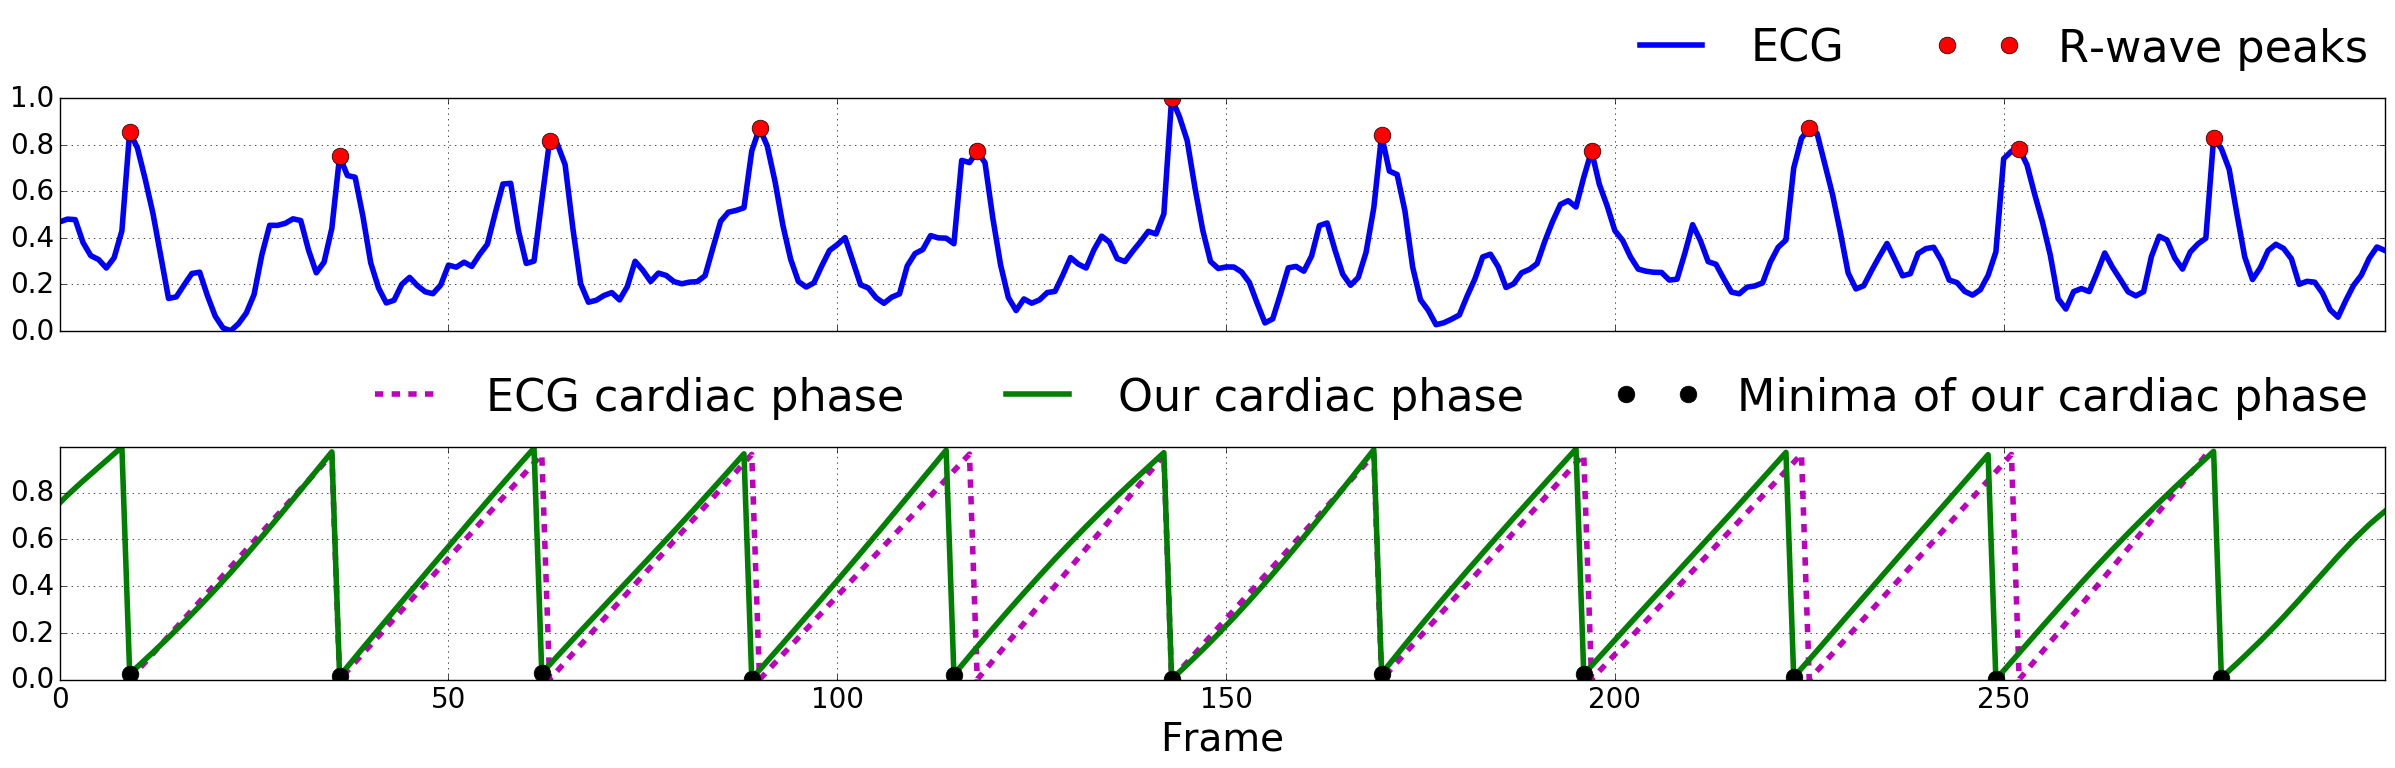
\includegraphics[width=7.0in]{figures/decoded/2015-07-27-10-36-06_2015-07-15-16-56-16_1.raw.bmode/ecg_instaphase_overlay.png}\\
\ionbox{7.0in}\\
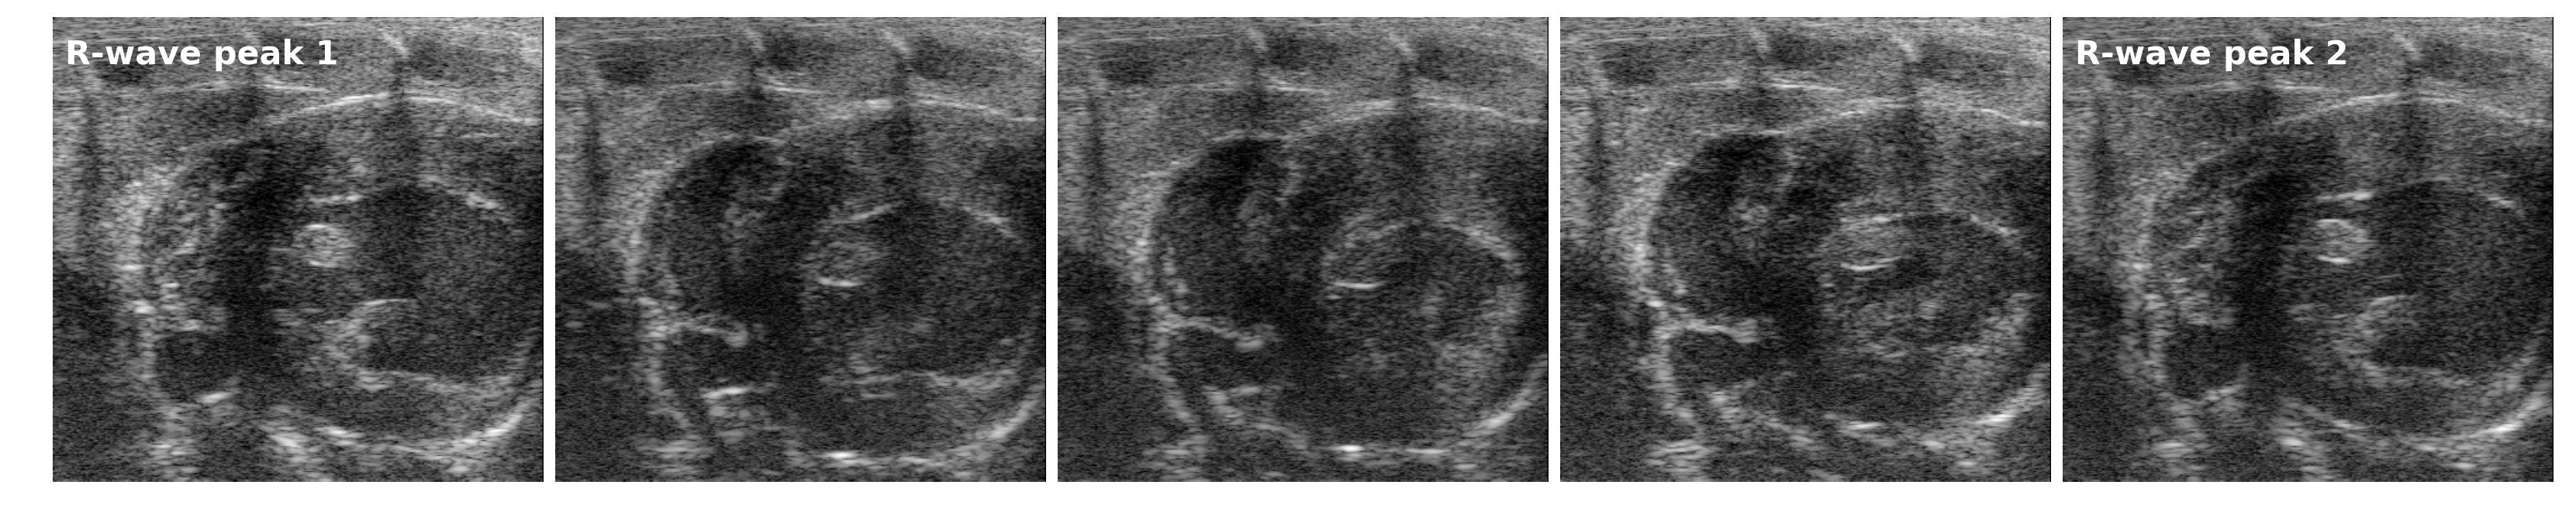
\includegraphics[width=7.0in]{figures/decoded/2015-07-27-10-36-06_2015-07-15-16-56-16_1.raw.bmode/qrs_peak_to_peak.png}\\
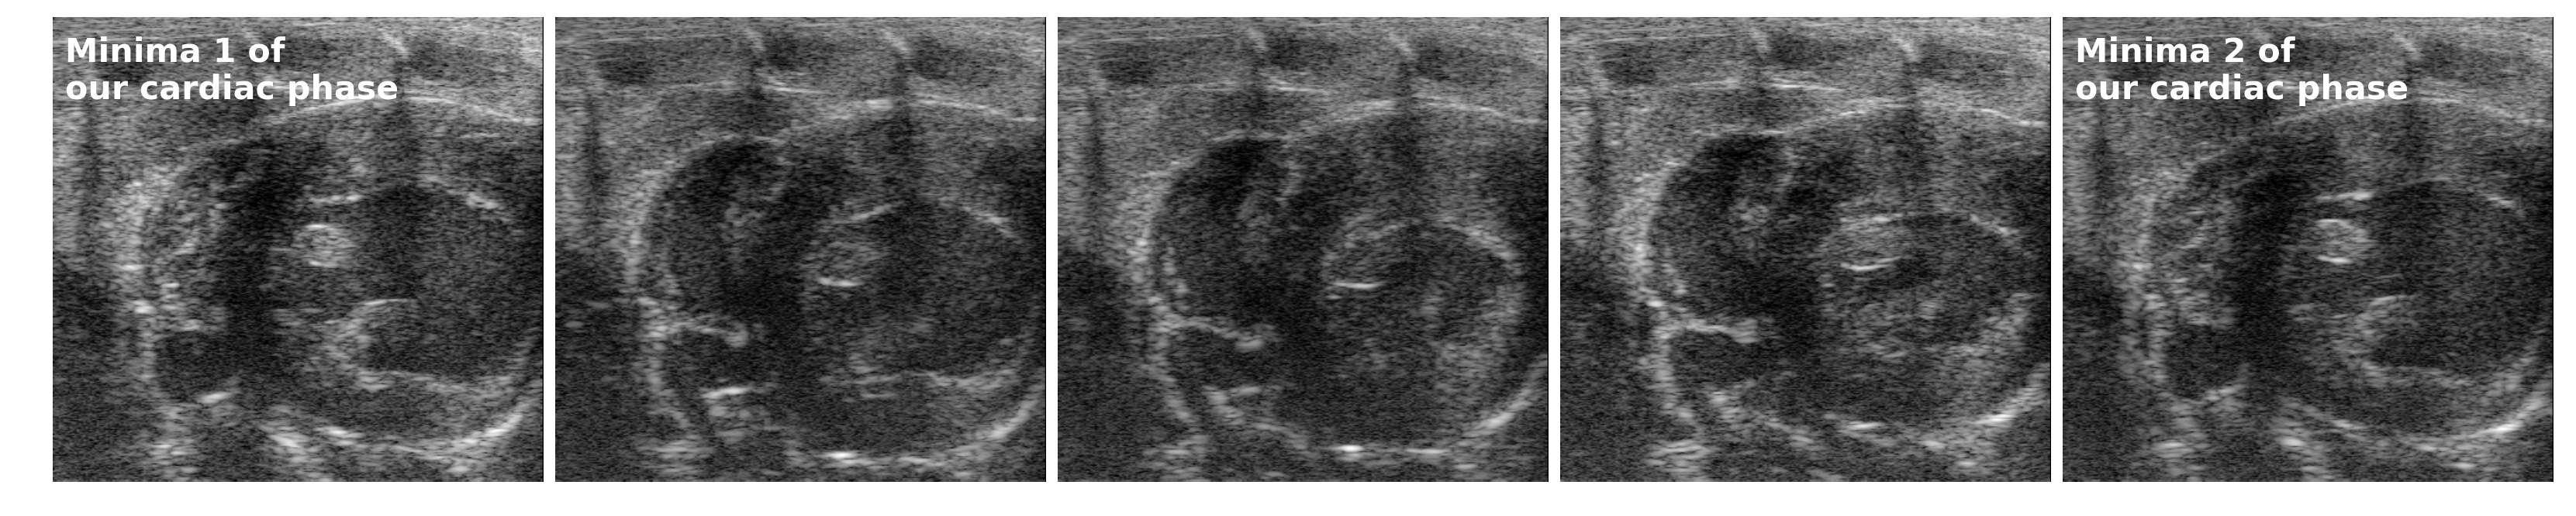
\includegraphics[width=7.0in]{figures/decoded/2015-07-27-10-36-06_2015-07-15-16-56-16_1.raw.bmode/instaphase_valley_to_valley.png}
\ionbox{7.0in}\\
%
\caption{Illustration of the close match between the cardiac phase derived from the ECG signal and the cardiac phase estimated using our method: (a) ECG signal simultaneously acquired with the image sequence (blue) overlaid with peaks of the R-wave in each cardiac cycle (red dot/circle), cardiac phase derived from the ECG signal (Pink dashed line) through linear interpolation between R-wave peaks~\cite{Rosenblum2001,Freund2003}, and the cardiac phase estimated directly from the image data using our method (green solid line) overlaid with the corresponding minima (black dot/circle), (b) Five video frames evenly spaced in time between the first and second R-wave peaks of the ECG signal (top-row) and the corresponding minima of the cardiac phase estimated using our method (bottom-row) constituting one cardiac cycle. Notice that the images in each column look very similar.}
\label{fig:instaphase_vs_ecg}
\end{figure*}
%

\vskip0.75ex
\noindent
\textbf{Related prior work.} Previous work on the estimation of cardiac and/or respiratory phases directly from ultrasound echocardiography videos is limited. In~\cite{Karadayi2006}, Karadayi\etal compute a signal of the x- or y-coordinate of the center-of-mass of each frame, use a band-pass filter to remove frequencies outside the cardiac range, determine the dominant frequency in the periodogram, and apply matched filtering using single-period sine and cosine signals at the dominant frequency to estimate the instantaneous cardiac phase. However, the center-of-mass signals may not be reliable in all scenarios. In~\cite{Sundar2009}, Sundar\etal compute a signal of phase correlation between consecutive frames and apply a band-pass and low-pass filter to obtain an estimate of the instantaneous cardiac and respiratory phase, respectively. Phase correlation encodes global translation in the image plane and cannot model out-of-plane motion of the beating heart present in our data. In~\cite{Wachinger2012}, Wachinger\etal use a manifold learning or non-linear dimensionality reduction technique called Laplacian Eigenmap to learn the low-dimensional manifold of the image sequence embedded in high-dimensional space and project the images onto the first eigen direction of the Laplacian of the image similarity graph to obtain a 1D signal encoding respiratory motion. In~\cite{Panayiotou2014}, Panayiotou\etal use a  series of image filtering operations to obtain a binary mask of pixels predominantly affected by cardiac/respiratory motion, apply a linear dimensionality reduction technique called principal component analysis (PCA) on the intensities of image pixels within the binary mask, project the images onto the principal directions with high variation to extract 1D signals encoding cardiac/respiratory motion, and post-process these signals by suppressing undesired frequencies in the frequency domain. While the aforementioned approaches based on manifold learning and masked PCA are promising and generally applicable, in this paper, we present a method that can estimate the cardiac phases more accurately. Instead of using dimensionality reduction methods such as PCA or manifold learning to implicitly derive intermediate representations decoupling the cardiac and respiratory motion, our method explicitly addresses this problem through a trend extraction technique that works directly on the inter-frame similarity in the original high-dimensional space. It then goes a step further and estimates the instantaneous cardiac and respiratory phases of each frame using a Hilbert transform approach that is shown to be less sensitive to small short-lived fluctuations\cite{Freund2003}.
%
%\vspace{-0.3cm}
%
\section{Method}
\label{sec:method}
%\vspace{-0.3cm}
%
In this section, we present the theory underlying the proposed methods along with visual illustrations of the intermediate results to help understand the underlying concepts. In Section~\ref{sec:method:phase_estimation}, we describe our method for estimation of instantaneous cardiac and respiratory phases  (Figure~\ref{fig:instaphase_vs_ecg}). In Section~\ref{sec:method:gating}, we present a robust method to exclude video frames with significant respiratory motion. In Section~\ref{sec:method:super_resolution}, we present a kernel regression model for reconstructing images at any cardiac phase facilitating temporal super-resolution.
%
%\vspace{-0.3cm}

\subsection{Estimation of cardiac and respiratory phases}
\label{sec:method:phase_estimation}
%
\begin{figure*}[!t]
\centering
\setcounter{lfigcounter}{1}
%
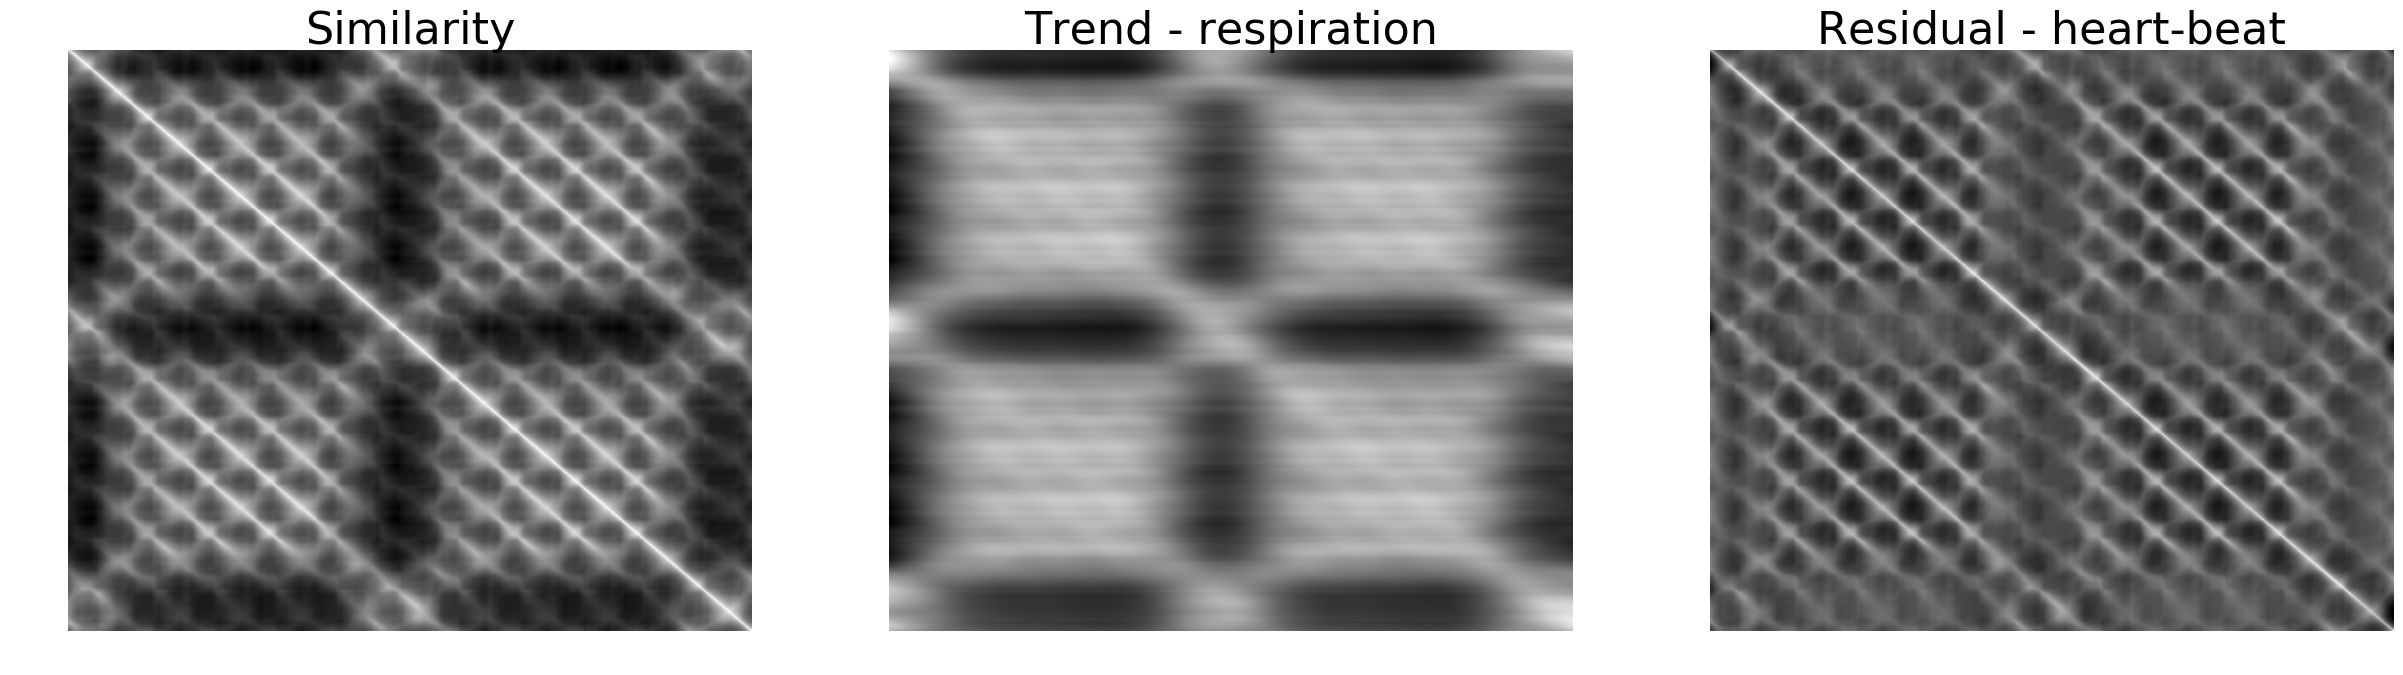
\includegraphics[width=6.0in]{figures/decoded/2015-07-27-10-36-06_2015-07-15-16-56-16_1.raw.bmode/simMat.png}
\ionbox{2in}\ionbox{2in}\ionbox{2in}\\
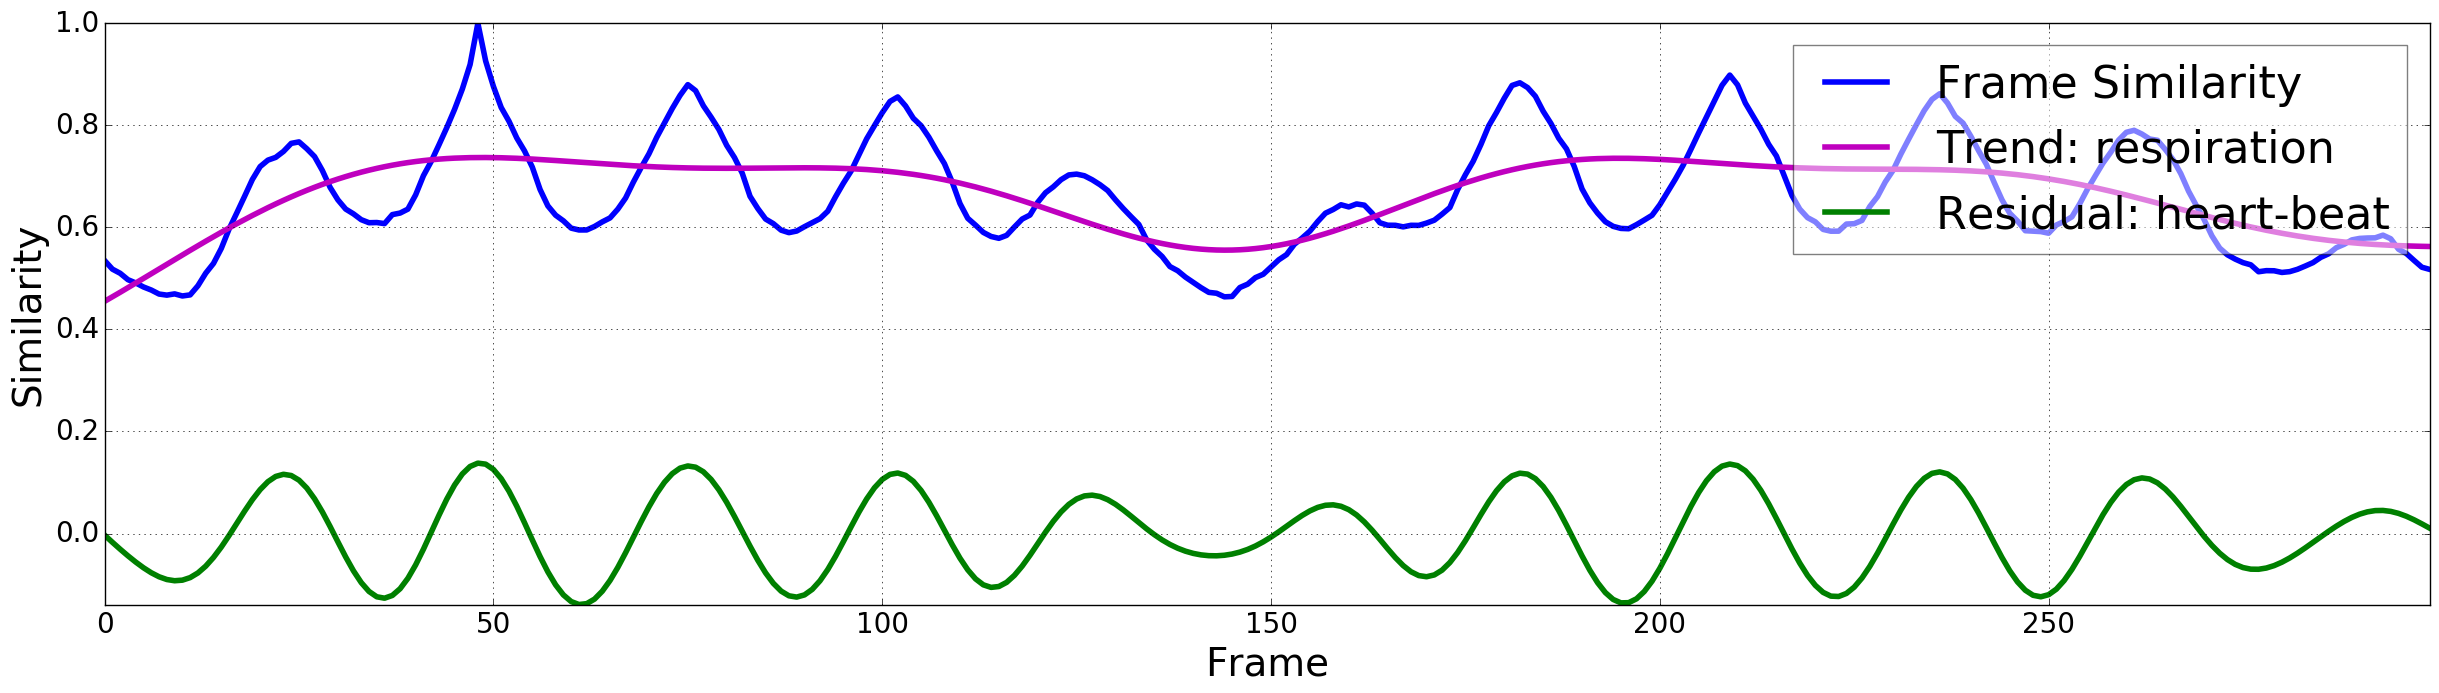
\includegraphics[width=6.0in]{figures/decoded/2015-07-27-10-36-06_2015-07-15-16-56-16_1.raw.bmode/season_trend_decomposition.png}
\ionbox{6.0in}\\
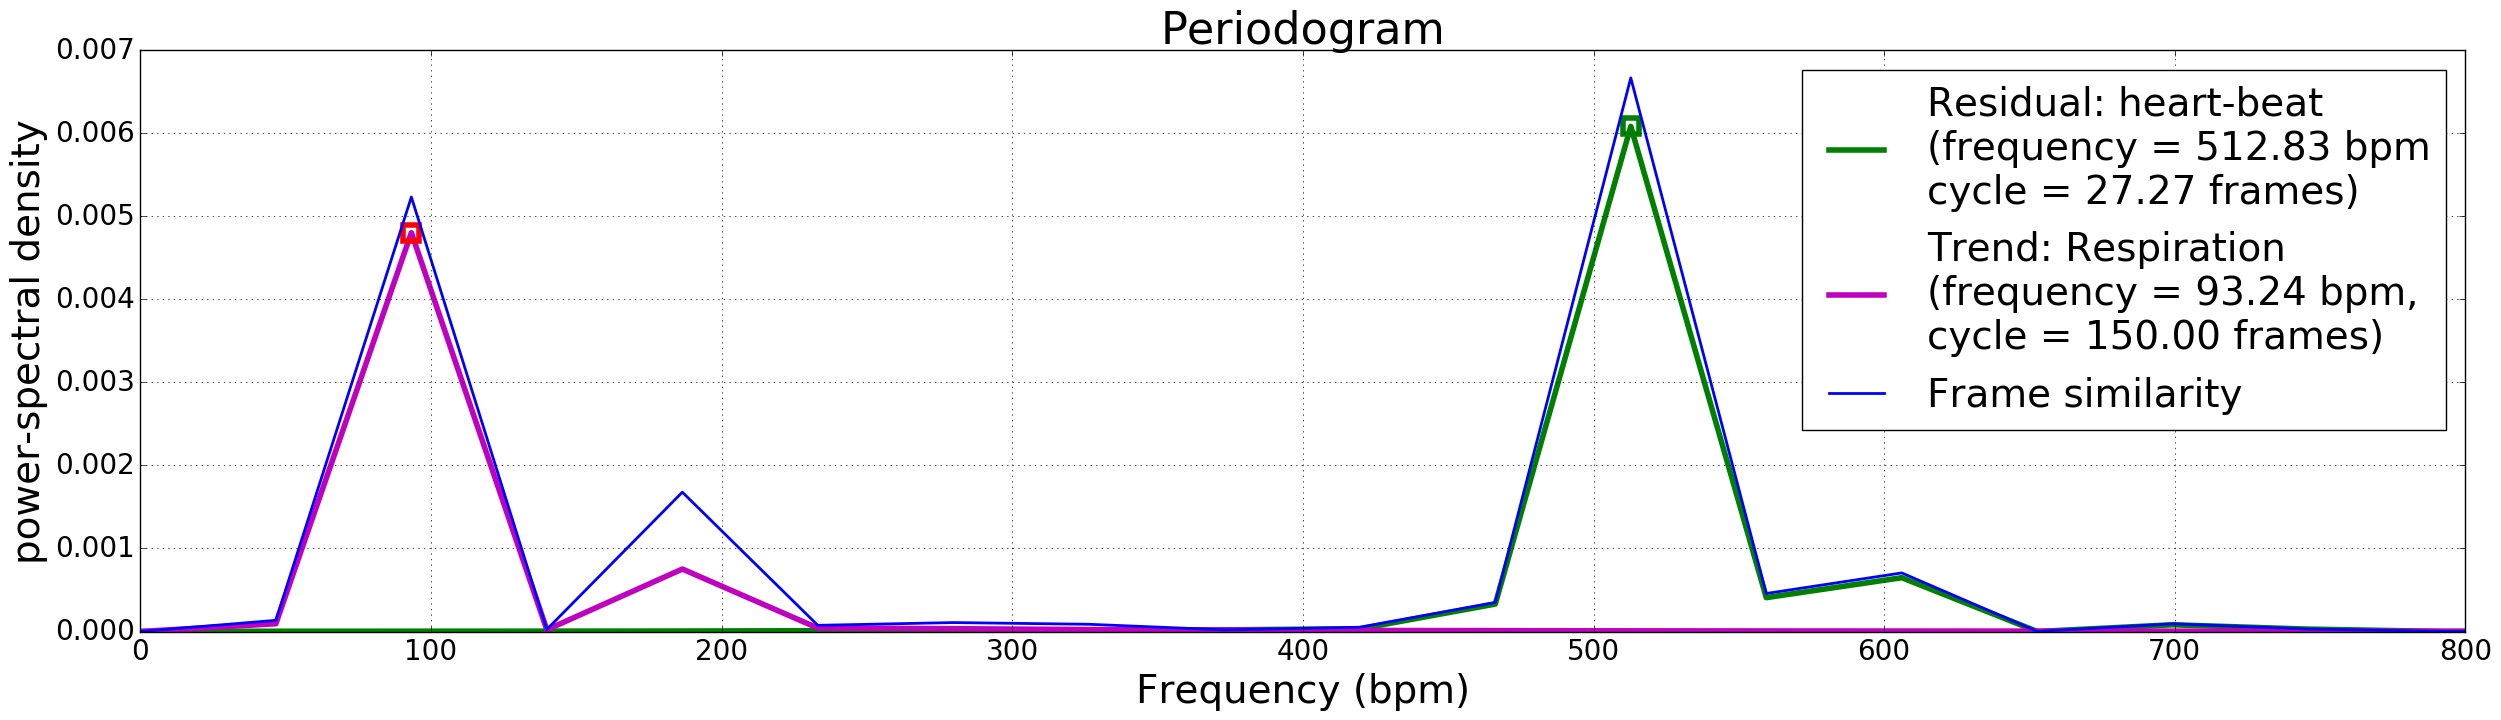
\includegraphics[width=6.0in]{figures/decoded/2015-07-27-10-36-06_2015-07-15-16-56-16_1.raw.bmode/periodogram.png}
\ionbox{6.0in}\\
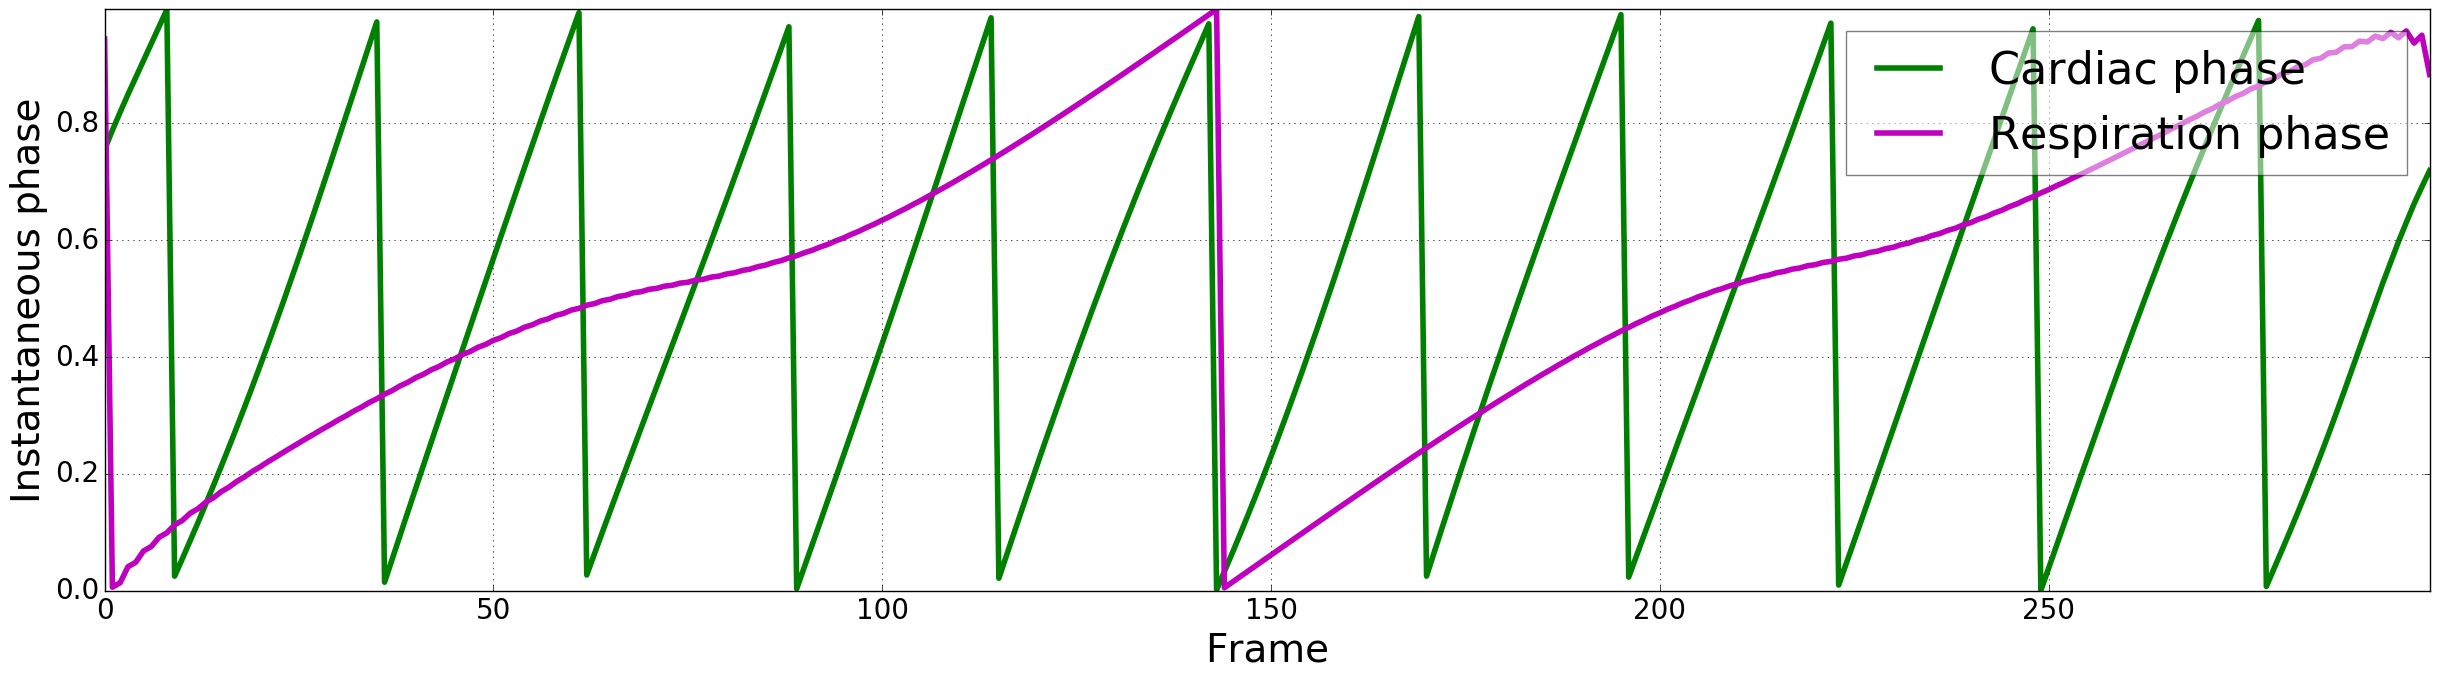
\includegraphics[width=6.0in]{figures/decoded/2015-07-27-10-36-06_2015-07-15-16-56-16_1.raw.bmode/instantaneous_phase.png}
\ionbox{6.0in}\\
%
\caption{Illustration of our phase estimation method: (a) Inter-frame similarity matrix, (b) Trend matrix corresponding to respiratory motion, (c) Residual matrix corresponding to beating heart motion, (d) Frame similarity $\hat{u}(t)$ selected for phase estimation with associated trend/respiration $\hat{\tau}_{resp}$ and residual/heart-beat $\hat{r}_{heart}$ signals, (e) Periodogram of heart-beat and respiration signals along with periodicity characteristics (e.g. frequency, cycle duration) calculated from the dominant frequency, and (f) Instantaneous cardiac and respiratory phases estimated using the Hilbert transform.}
\label{fig:phase_estimation}
\end{figure*}
%

While there have been numerous efforts for the estimation of instantaneous phase and/or frequency in periodic univariate time series data~\cite{Boashash1992,Rosenblum2001,Freund2003,Luo2003,Lu2013}, there are not many methods that tackle this problem in a multivariate setting such as the case of cardiac ultrasound videos wherein thousands of variables (pixel intensities) are involved. Our strategy is to transform this complex multivariate problem into a univariate one and take advantage of existing methods to solve the problem. 
%
\begin{figure*}[t]
\centering
\setcounter{lfigcounter}{1}
%
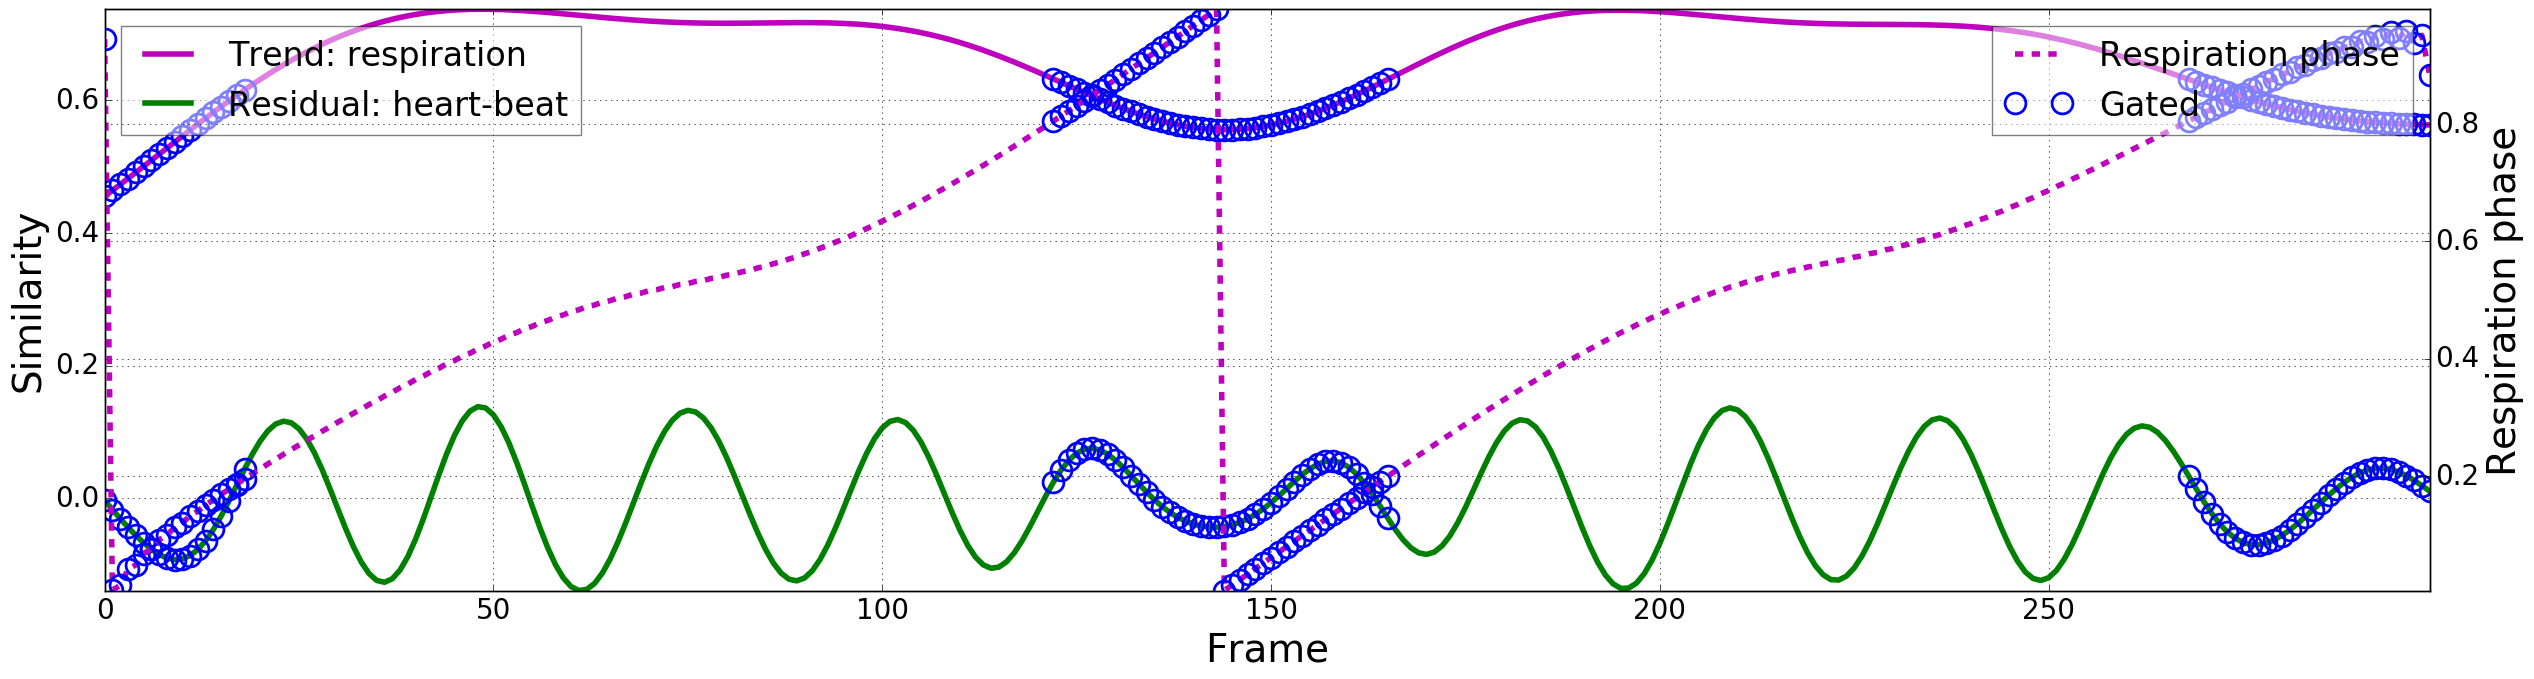
\includegraphics[width=6.8in]{figures/decoded/2015-07-27-10-36-06_2015-07-15-16-56-16_1.raw.bmode/respiratory_phase_gating.png}
\ionbox{7.0in}\\
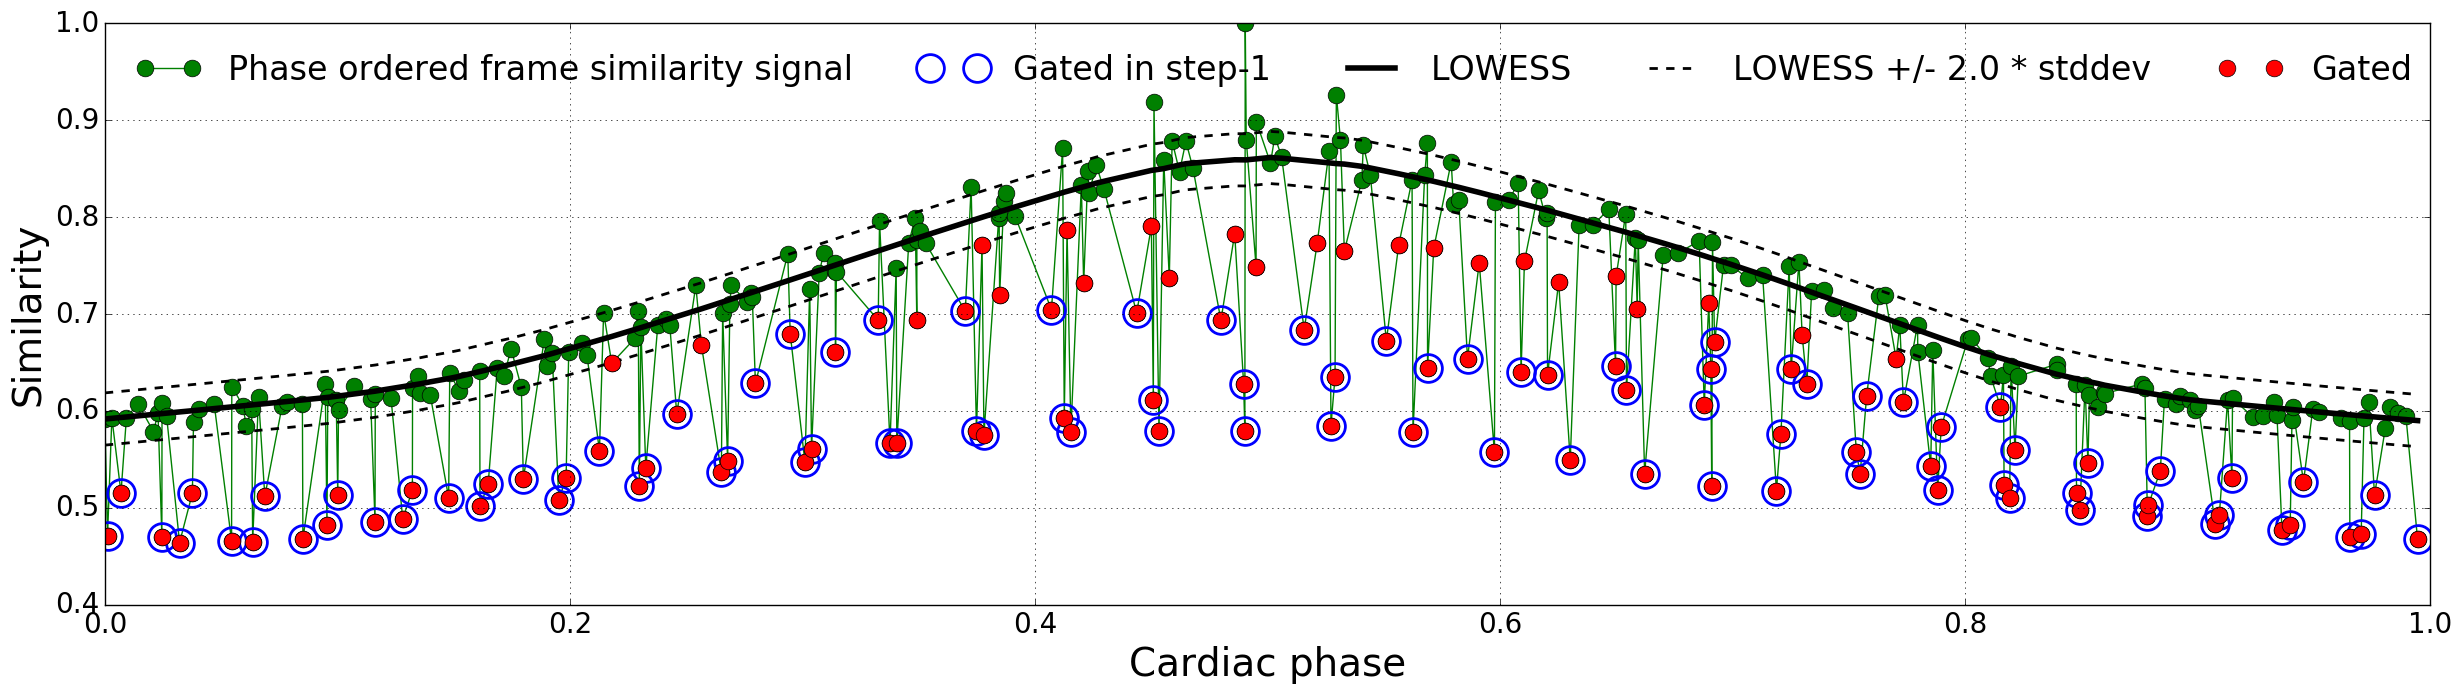
\includegraphics[width=6.8in]{figures/decoded/2015-07-27-10-36-06_2015-07-15-16-56-16_1.raw.bmode/robust_lowess_gating.png}
\ionbox{7.0in}\\
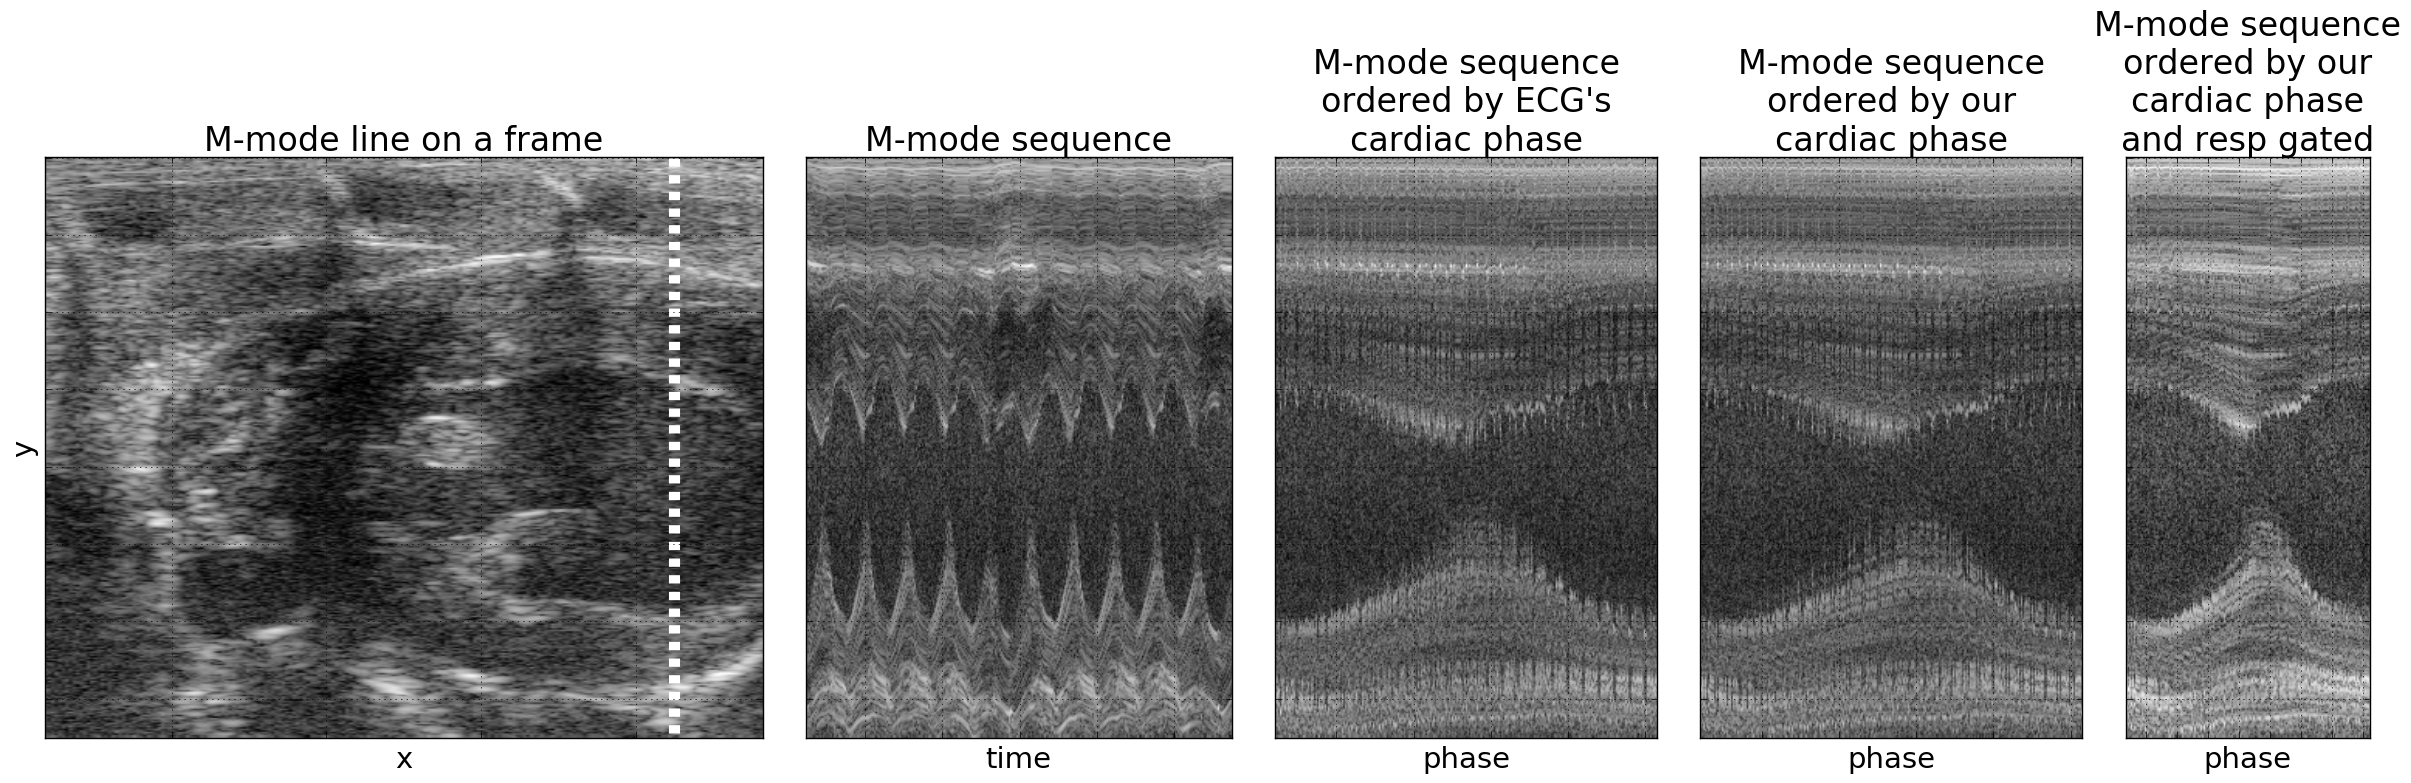
\includegraphics[width=6.8in]{figures/decoded/2015-07-27-10-36-06_2015-07-15-16-56-16_1.raw.bmode/phaseordered.png}
\ionbox{2.3in}\ionbox{1.3in}\ionbox{1.2in}\ionbox{1.2in}\ionbox{0.8in}\\
%
\caption{Illustration of the respiratory gating method: (a) Frames $F_{cutoff}$ discarded (blue circles) in step-1 overlaid with the respiration $\hat{\tau}_{resp}(t)$, heart-beat $\hat{r}_{heart}(t)$, and respiratory phase $\hat{\phi}_{resp}(t)$ signals, (b) The frame similarity signal $\hat{u}(t)$ vs cardiac phase $\hat{\phi}_{heart}(t)$ overlaid with frames $F_{cutoff}$ discarded in step-1 (blue circles), LOWESS fit $L(\phi_{heart})$ (black solid lines), upper and lower bounds or 95\% confidence interval $(L(\phi_{heart}) \pm 2.0 * \hat{\sigma}_L)$ of non-respiratory frames around the LOWESS fit (black dotted line), and frames $F_{resp}$ (red circles) gated after step-2, (c) One of the frames in one of our cardiac ultrasound videos overlaid with the M-mode line shown in the next four images to the right, (d) M-mode frames in the order they appear in the input video, (e) M-mode frames ordered by cardiac phase derived from the ECG signal, (f,g) M-mode frames ordered by cardiac phase estimated using our method before and after dropping the frames with heavy respiratory motion spotted by our respiratory gating technique.}
\label{fig:respiratory_gating}
\end{figure*}
%

We first compute the similarity between all pairs of images/frames in the given quasi-periodic image sequence containing $N$ frames to create a symmetric matrix $S \in R^{N \times N}$ wherein the element $S(i,j)$ is equal to the similarity between the $i^{th}$ and $j^{th}$ frame. \rk{Each row in the inter-frame similarity matrix $S$ can now be seen as a univariate time series. The inter-frame similarity metric must be chosen such that this time series preserves the periodicity characteristics of cardiorespiratory motion in the original image sequence. Here, we use normalized correlation to quantify inter-frame similarity; but in principle, other image similarity metrics can be used~\cite{Yoo2004}. Figure~\ref{fig:phase_estimation}(a) shows the inter-frame similarity matrix of one of our cardiac ultrasound videos wherein the periodicity characteristics of low-frequency respiratory motion and high-frequency beating heart motion can be observed. Notice that the rows of this matrix appear to be a superposition of two near-sinusoidal signals with the periodic signatures of cardiac and respiratory motion, respectively}.

Next, we use a trend extraction technique called the Hodrick-Prescott (HP) filter~\cite{Alexandrov2012} to decouple the periodic signatures of cardiac and respiratory motions from the frame similarity signal $u^i(t)$ corresponding to each row $i$ of the matrix $S$ by decomposing it into a sum of two components: (i) lower frequency trend component $\tau^i_{resp}(t)$ with periodicity characteristic of only respiratory motion, and (ii) higher frequency residual component $r^i_{heart}(t)$ with periodicity characteristic of only beating heart motion. The HP filter performs the decomposition of $u^i(t) = \tau^i_{resp}(t) + r^i_{heart}(t)$ by solving the following optimization problem:
\begin{equation}	
\argmin{\tau^i_{resp}(t)} \sum_{t=1}^{N}  \left(u^i(t) - \tau^i_{resp}(t) \right)^2  + \lambda \sum_{t=1}^{N-1} \left( \nabla^2 \tau^i_{resp}(t) \right)^2
\end{equation}
where $\nabla^2\tau^i_{resp}(t) = \tau^i_{resp}(t+1) - 2 \tau^i_{resp}(t) + \tau^i_{resp}(t-1)$ is the second-order difference or derivative of the trend signal and $\lambda$ is a penalty parameter that is set to 6400 which empirically resulted in a good separation between the periodograms or power-frequency distributions of the resulting trend and residual component signals. Let $S_{resp}$ and $S_{heart}$ be the matrices whose rows contain the trend/respiratory and residual/heart-beat components (Figures~\ref{fig:phase_estimation}(b,c)), respectively, of the frame similarity signal in the corresponding rows of matrix $S$. \rk{We then select the trend/respiratory and residual/heart-beat component signals corresponding to one of the rows in $S$ for phase estimation. A natural question that arises now is which of these rows would be a better choice for phase estimation. We devised a procedure to make this choice objective based on the notion that if the HP filter was successful in decoupling the periodic signatures of cardiac and respiratory motion, then the resulting trend/respiratory and residual/heart-beat component signals must be as near-sinusoidal or narrow-banded as possible. For each row in the inter-frame similarity matrix $S$, we compute the periodogram or power-frequency distribution of its heart-beat component signal, normalize it to sum to 1 such that it can be treated as a probability distribution, and compute its entropy. The smaller this entropy value, the more narrow banded or near-sinusoidal it would be. Hence, we select the row with the smallest entropy value. Let $\hat{u}(t)$ be the frame similarity signal of the selected row and let $\hat{\tau}_{resp}(t)$ and $\hat{r}_{heart}(t)$  be its associated trend and residual components  (Figure~\ref{fig:phase_estimation}(d)) that we will henceforth refer to as respiration and heart-beat signals, respectively}. To suppress undesired frequencies, we apply a low-pass filter with a typical mice respiration cutoff frequency of 230 BPM to the respiration signal $\hat{\tau}_{resp}(t)$ and a band-pass filter within the typical mice heart frequency range of 310-840 BPM to the heart-beat signal $\hat{r}_{heart}(t)$.

Next, considering the narrow-band near-sinusoidal nature of the respiration and heart-beat signals (Figure~\ref{fig:phase_estimation}(e)), we use the concept of the analytic signal involving the Hilbert transform as introduced by Gabor to estimate the instantaneous phase of each frame~\cite{Gabor1946,Bracewell1986,Rosenblum2001,Freund2003,Kuklik2015}. Specifically, we compute the instantaneous phase $\phi(t) \in \left [  -\pi, \pi\right )$ of a periodic time series $x(t)$ to be the instantaneous phase of its analytic signal $A_x(t) = x(t) + i H_x(t)$ involving its Hilbert transform $H_x(t)$ as follows: $\phi(t) = arctan \left( \frac{H_x(t)}{x(t)}\right)$ and map $\phi(t)$ from $\left [  -\pi, \pi\right )$ to $\left [  0, 1\right )$. Let $\hat{\phi}_{heart}(t)$ and $\hat{\phi}_{resp}(t)$ denote the instantaneous cardiac and respiratory phases (Figure~\ref{fig:phase_estimation}(f)) computed from the respiration and heart-beat signals, respectively.
%
%\vspace{-0.3cm}
\subsection{Gating out respiratory frames}
\label{sec:method:gating}
%
Once the cardiac and respiratory phases of each frame have been estimated, they can be used to select or filter out frames from a desired part/point in the periodic cycle, a process commonly referred to as gating. In this section, we present a robust two-step method that uses these phase estimates to filter out video frames with significant respiratory motion to enable the creation of an image sequence containing only cardiac motion.

In the first step, based on the observation that heaviest amount of the respiratory motion occurs within a short interval around the minima of the respiration signal $\hat{\tau}_{resp}(t)$ (pink curve in Fig.~\ref{fig:phase_estimation}(d)) with respiratory phase $\hat{\phi}_{resp}(t) = 0$, we perform a rough initial gating by discarding the frames $F_{cutoff} = \left \{ t \mid \hat{\phi}_{resp}(t) < c \vee \hat{\phi}_{resp}(t) > (1 - c) \right \}$ whose phase distance from $\hat{\phi}_{resp}(t) = 0$ is below a specified cutoff value $c=0.2$ chosen empirically. Figure~\ref{fig:respiratory_gating}(a) shows the discarded frames $F_{cutoff}$ overlaid on the respiration $\hat{\tau}_{resp}(t)$, heart-beat  $\hat{r}_{heart}(t)$, and respiratory phase $\hat{\phi}_{resp}(t)$ signals.

In the second step, we learn a regression function $L(\phi_{heart}) : \left [  0, 1\right ) \to R$ to predict the frame similarity signal value for any cardiac phase by fitting a robust non-parametric regression model called Locally Weighted Regression (LOWESS)~\cite{Cleveland1988} to the dataset $\left \{ \left(\hat{\phi}_{heart}(t), \hat{u}(t) \right) \mid \forall t \notin F_{cutoff}  \right \}$ containing the pair of the cardiac phase $\hat{\phi}_{heart}(t)$ and frame similarity signal $\hat{u}(t)$  values of all frames that do not belong to the set of frames $F_{cutoff}$ discarded in the first step above. \rk{Given any cardiac phase, LOWESS regression takes k-nearest training samples based on their cardiac phase values and uses  iterative weighted linear regression to predict the corresponding frame similarity signal value. This local fitting approach enables LOWESS regression to model a much wider class of functions than is possible with parametric approaches such as polynomial regression}. Next, we compute a robust estimate of the standard deviation $\hat{\sigma}_{L}$ of non-respiratory frames around the LOWESS fit based on the median absolute deviation between the LOWESS fit $L( \hat{\phi}_{heart}(t) )$ and frame similarity signal $\hat{u}(t)$ for all frames. Lastly, we gate out all frames $F_{resp} = \left \{ t : \lvert \hat{u}(t) - L( \hat{\phi}_{heart}(t) ) \rvert   > k \times \hat{\sigma}_{L}  \right \}$ whose frame similarity signal value deviates from the LOWESS fit by more than $k = 2.0$ (95\% confidence interval) times the standard deviation $\hat{\sigma}_{L}$ (Figure~\ref{fig:respiratory_gating}(b)). Figure~\ref{fig:respiratory_gating}(d) shows an m-mode view of one of our videos along the m-mode line shown in Figure~\ref{fig:respiratory_gating}(c). Figures~\ref{fig:respiratory_gating}(e,f) show the m-mode sequence ordered by the cardiac phase derived from the ECG signal and the cardiac phase estimated using our method, respectively, that look very similar. Notice the jaggedness/discontinuities along the horizontal direction at chamber wall in both these images that is caused by large movements induced by respiratory motion. Figure~\ref{fig:respiratory_gating}(g) shows the result obtained by ordering the m-mode sequence by the cardiac phase estimated using our method and gating out the respiratory frames using the method described above. Notice the significant reduction in the jaggedness/discontinuities after gating out or discarding the frames with heavy respiratory motion.
%
%\vspace{-0.3cm}
\subsection{Model to reconstruct images by cardiac phase}
\label{sec:method:super_resolution}
%
%
\begin{figure*}[t]
\centering
\setcounter{lfigcounter}{1}
%
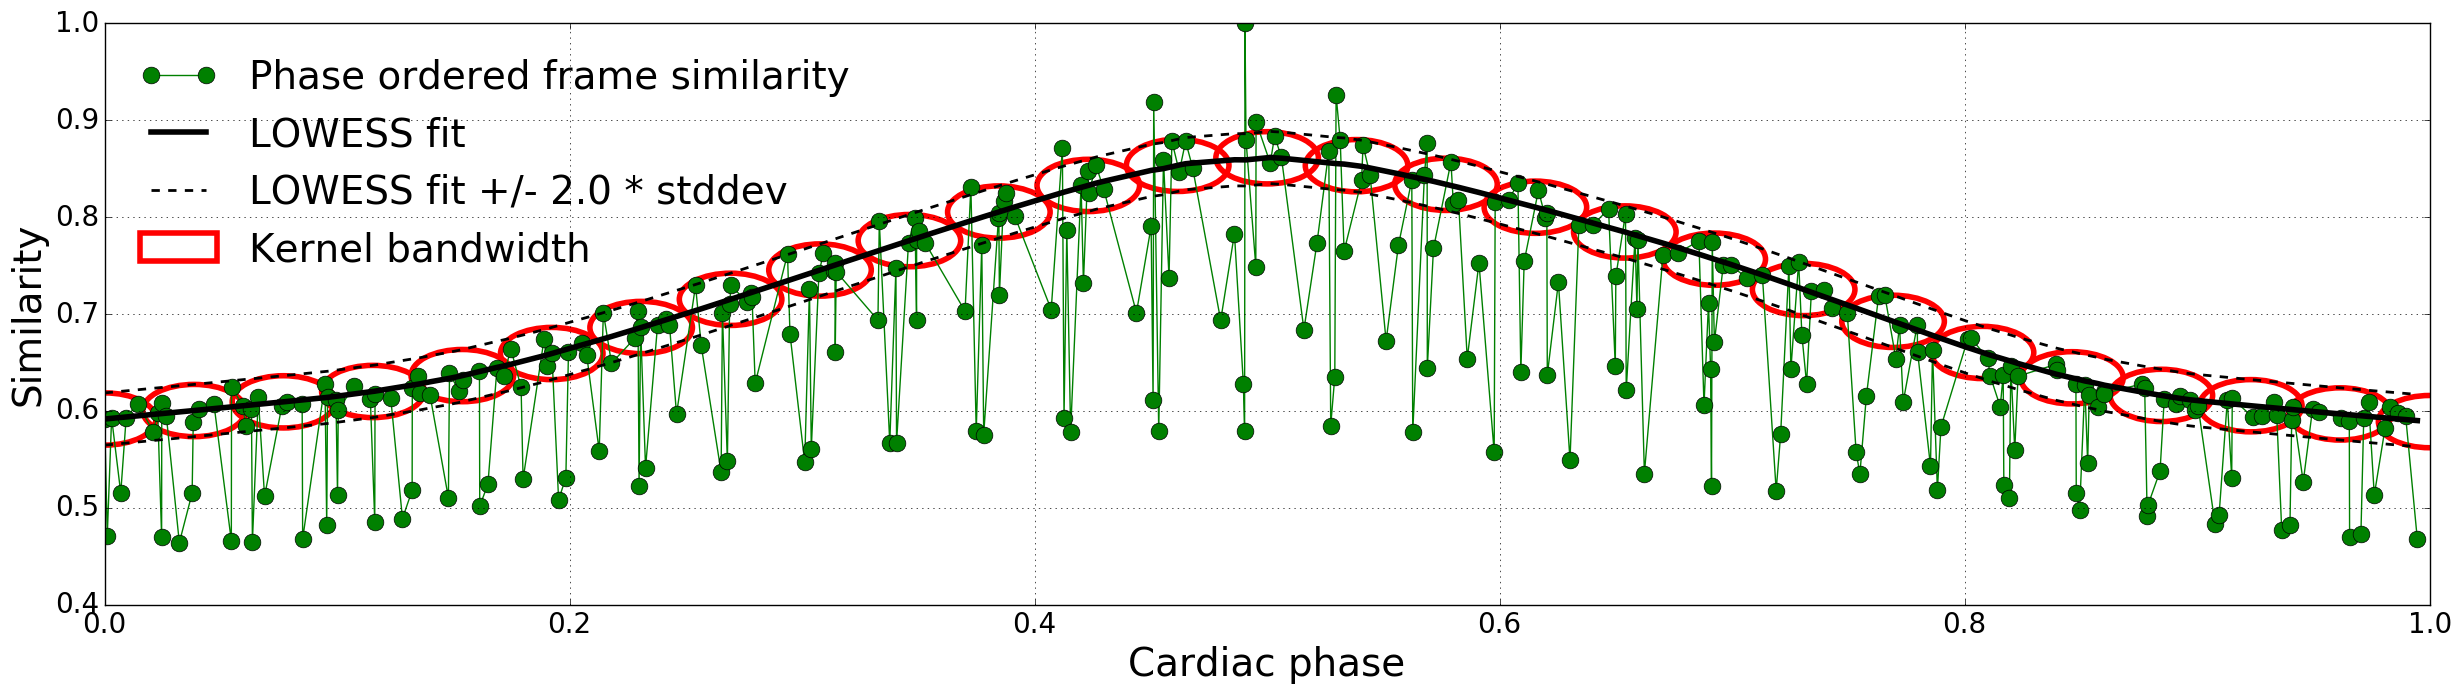
\includegraphics[width=6.8in]{figures/decoded/2015-07-27-10-36-06_2015-07-15-16-56-16_1.raw.bmode/phase_similarity_bandwidth.png}\\
\ionbox{6.8in}\\
\vspace{0.3cm}
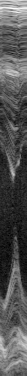
\includegraphics[height=2.5in]{figures/decoded/2015-07-27-10-36-06_2015-07-15-16-56-16_1.raw.bmode/Input_Mag_1_kernel_regression_phase_sim.png}
\hspace{0.02cm}
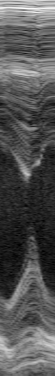
\includegraphics[height=2.5in]{figures/decoded/2015-07-27-10-36-06_2015-07-15-16-56-16_1.raw.bmode/Input_Mag_2_kernel_regression_phase_sim.png}
\hspace{0.02cm}
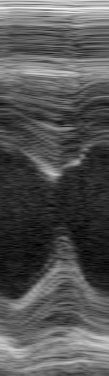
\includegraphics[height=2.5in]{figures/decoded/2015-07-27-10-36-06_2015-07-15-16-56-16_1.raw.bmode/Input_Mag_4_kernel_regression_phase_sim.png}
\hspace{0.02cm}
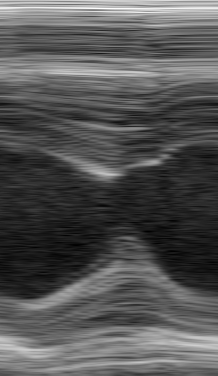
\includegraphics[height=2.5in]
{figures/decoded/2015-07-27-10-36-06_2015-07-15-16-56-16_1.raw.bmode/Input_Mag_8_kernel_regression_phase_sim.png}
\hspace{1.0cm}
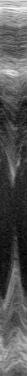
\includegraphics[height=2.5in]{figures/decoded/2015-07-27-10-36-06_2015-07-15-16-56-16_1.raw.bmode/Input_Mag_1_kernel_regression_phase.png}
\hspace{0.02cm}
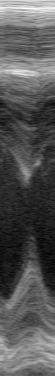
\includegraphics[height=2.5in]{figures/decoded/2015-07-27-10-36-06_2015-07-15-16-56-16_1.raw.bmode/Input_Mag_2_kernel_regression_phase.png}
\hspace{0.02cm}
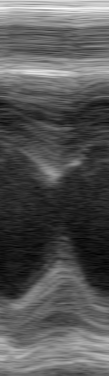
\includegraphics[height=2.5in]{figures/decoded/2015-07-27-10-36-06_2015-07-15-16-56-16_1.raw.bmode/Input_Mag_4_kernel_regression_phase.png}
\hspace{0.02cm}
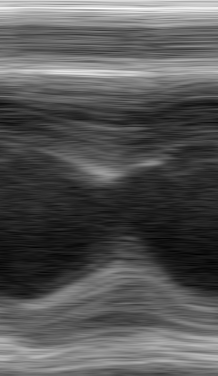
\includegraphics[height=2.5in]
{figures/decoded/2015-07-27-10-36-06_2015-07-15-16-56-16_1.raw.bmode/Input_Mag_8_kernel_regression_phase.png}\\
\ionbox{3.5in}\ionbox{3.5in}\\
%
\caption{Illustration of temporal super-resolution using our kernel regression model: (a) Shows the frame similarity signal $\hat{u}(t)$ vs cardiac phase $\hat{\phi}_{heart}(t)$ overlaid with LOWESS fit $L(\phi_{heart})$ (black solid lines), upper and lower bounds or 95\% confidence interval $(L(\phi_{heart}) \pm 2.0 * \sigma_L)$ of non-respiratory frames (black dotted lines), and the kernel bandwidth shown at a series of cardiac phases as red ellipses whose length along the phase and similarity axis is set to $\sigma_\phi$ and $\hat{\sigma}_{L}$ as described in Section~\ref{sec:method:super_resolution}, (b) M-mode views of single cardiac cycle videos reconstructed at 1x, 2x, 4x, and 8x temporal magnification using our NW kernel regression model with a bivariate kernel defined in both cardiac phase and frame similarity space, (c) M-mode views of single cardiac cycle videos reconstructed at 1x, 2x, 4x, and 8x temporal magnification using the NW kernel regression model with a kernel defined in cardiac phase space only.}
\label{fig:phase_similarity_bandwidth}
\end{figure*}
%
In this section, we present a kernel regression model to reconstruct the image at any cardiac phase. This model can then be used to generate a single-cycle video representative of the subject's heart-beat at a higher temporal resolution from a low-frame rate video of multiple heart beats. Given a cardiac ultrasound video $I(t) : \{1, ..., N\} \to R^m$ of $N$ frames with $m$ pixels each, we estimate the instantaneous cardiac phase $\hat{\phi}_{heart}(t)$ of each frame and compute the robust LOWESS fit $L(\phi_{heart}) : \left [  0, 1\right ) \to R$ that maps cardiac phase to its frame similarity signal value as described in Sections~\ref{sec:method:phase_estimation} and ~\ref{sec:method:gating}. We then use Nadarya-Watson (NW) kernel regression \cite{Bishop2006} to learn a function $M(\phi_{heart}): [0, 1) \to R^m $ that reconstructs the image for any cardiac phase $\phi$ using a kernel-weighted local average as follows:
\begin{equation}
M(\phi_{heart}) = \frac{\sum_{t = 1}^{N} K \left( \phi_{heart}, \hat{\phi}_{heart}(t) \right) I(t)}{\sum_{t = 1}^{n} K \left( \phi_{heart}, \hat{\phi}_{heart}(t) \right)} 
\end{equation}
wherein we define the kernel $K\left( \phi_{heart}, \hat{\phi}_{heart}(t) \right) = exp\left \{ -\frac{ \mid \phi_{heart} - \hat{\phi}_{heart}(t) \mid^2}{2  \sigma^2_\phi} \right \} \times exp\left \{ -\frac{ \mid L(\phi_{heart}) - \hat{u}(t) \mid^2}{2  \sigma^2_{L}} \right \}$ as the product of two radial-basis function (RBF) kernels. The first RBF kernel gives higher weights to images whose cardiac phase is closer (accounting for periodicity) to the target phase. Its bandwidth $\sigma_\phi$ is set equal to a constant $k_\phi = 0.4$ times the median difference in cardiac phase between consecutive frames of the given image sequence. The second RBF kernel gives higher weights to images whose frame similarity signal value is close to the LOWESS prediction $L(\phi_{heart})$. Its bandwidth $\sigma_{L}$ is set equal to a constant $k_L = 2.0$ times the robust estimate of standard deviation $\hat{\sigma}_{L}$ of non-respiratory frames ($\forall t \notin F_{resp}$) around the LOWESS fit. As a result of this, frames with heavy respiratory motion will get very low weight values even if their cardiac phase is similar to the target phase. Figure~\ref{fig:phase_similarity_bandwidth}(a) shows bandwidth of the kernel in phase and similarity space computed as described above. The model $M(\phi_{heart})$ can now be used to reconstruct a single-cycle video representative of the subject's heart-beat by generating images at any desired resolution/sampling of phases in the range $[0, 1)$.  \rk{Figure~\ref{fig:phase_similarity_bandwidth}(b) shows m-mode views of the single-cycle videos reconstructed at 1x, 2x, 4x, and 8x temporal magnification using the NW kernel regression model with a bivariate RBF kernel defined in both cardiac phase and frame similarity space. For comparison,  Figure~\ref{fig:phase_similarity_bandwidth}(c) shows m-mode views of the reconstructions obtained with a univariate RBF kernel defined in cardiac phase space only}. 
%
%\vspace{-0.3cm}
\section{Experimental Data and Results}
\label{sec:results}
%\vspace{-0.3cm}
%
We used 2D cardiac ultrasound or echocardiography videos and simultaneously captured ECG recordings of 6 mice to validate our methods. The ultrasound videos were acquired using the VisualSonics Vevo 2100 scanner at 233 frames per second (FPS). Each video consists of approximately 300 frames, 11 cardiac cycles, and 2 respiratory cycles.

We validated the cardiac phase estimates of our method by comparing them with the cardiac phase derived from the ECG signal which is the gold standard for cardiac gating. Figure~\ref{fig:instaphase_vs_ecg}(a) presents a visual comparison between the instantaneous cardiac phase derived from the ECG signal through linear interpolation between R-wave peaks~\cite{Rosenblum2001,Freund2003} and the instantaneous cardiac phase estimated directly from the image data using our method on one of the 6 videos. Figure~\ref{fig:instaphase_vs_ecg}(b) presents a visual comparison of five video frames evenly spaced in time between two consecutive R-wave peaks of the ECG signal (top-row) and the corresponding minima of the cardiac phase signal computed using our method (bottom-row). Table~\ref{table:phase_estimation_error} reports statistics of the error between the cardiac phases estimated by our method and the cardiac phases derived from the ECG signal for all the 6 videos \rk{where in the phases are in the normalized $[0, 1]$ range}. The supplementary material includes a video showing the cardiac and respiratory phases of each frame estimated using our method for one of the 6 videos.

%	
\begin{table}[h]
\begin{minipage}[t]{0.95\linewidth}
\centering
\caption{Error between the cardiac phases estimated using our method and those obtained from the ECG signal.}
%%\vspace{-0.1cm}
\begin{tabular}{|c|c|c|c|c|}
\hline
VID & mean $\pm$ stddev & median & IQR & range \\ \hline
1 & 0.06 $\pm$ 0.03 & 0.06 & 0.05 & {[}0.00, 0.14{]} \\ \hline
2 & 0.06 $\pm$ 0.03 & 0.05 & 0.05 & {[}0.00, 0.12{]} \\ \hline
3 & 0.06 $\pm$ 0.03 & 0.06 & 0.06 & {[}0.00, 0.12{]} \\ \hline
4 & 0.04 $\pm$ 0.02 & 0.04 & 0.02 & {[}0.00, 0.10{]} \\ \hline
5 & 0.06 $\pm$ 0.03 & 0.06 & 0.03 & {[}0.00, 0.12{]} \\ \hline
6 & 0.03 $\pm$ 0.02 & 0.04 & 0.03 & {[}0.00, 0.05{]} \\ \hline \hline
Average & 0.05 $\pm$ 0.03 & 0.05 & 0.04 & {[}0.00, 0.11{]} \\ \hline
\end{tabular}
\label{table:phase_estimation_error}
\end{minipage}
\end{table}	
%	
	
We also compared the performance of our phase estimation method with three previously published methods, namely: Phase correlation approach of Sundar\etal\cite{Sundar2009}, Manifold learning approach of Wachinger\etal\cite{Wachinger2012}, and the Masked PCA approach of Panayiotou\etal\cite{Panayiotou2014}. For the phase correlation approach, we applied a bandpass filter in the mice cardiac frequency range (310-840 bpm) to the phase correlation signal to extract the cardiac signal. For the manifold learning approach, we project the high-dimensional image sequence onto the second principal direction and apply a band-pass filter in the mice cardiac frequency range (310-840 bpm) to extract the cardiac signal. For the Masked PCA approach, we compute the binary mask by thresholding the response of Frangi's vesselness filter tuned to enhance the moving heart chamber walls that look like ridges, perform PCA on the intensities of pixels within the binary mask,  project the high-dimensional image sequence onto the second principal direction (projection onto the first principal direction only encodes respiratory motion in our data), and apply a band-pass filter in the mice cardiac frequency range to extract the cardiac signal. Note that each of these three prior works only propose a method for deriving a 1D signal reflecting the periodicity characteristics of the cardiac/respiratory motion in the given image sequence. They do not provide an approach to compute the instantaneous phase from the derived signal. Hence, we compare the performance of these methods with ours in localizing the R-wave peaks of the ECG signal that corresponds to the peaks/valleys of the 1D signals derived by these methods. Table~\ref{table:R_peak_localization} reports the $mean \pm stddev$ frame error of different methods in locating the video frames corresponding to the R-wave peaks of the ECG signal for all 6 videos \rk{where in the result of the best performing method for each video is highlighted in bold}. Note that the duration of the time interval between two consecutive frames is 4.29 ms and the average length of cardiac cycle in our videos is 27.27 frames or 116.98 ms.
	
%	
\begin{table}[h]
\begin{minipage}[t]{0.95\linewidth}
\centering
\caption{Error in localization of the frames corresponding to the peaks of the R-wave in ECG signal using different methods.}
%%\vspace{-0.1cm}
\setlength\tabcolsep{3pt} 
\begin{tabular}{|c|c|c|c|c|}
\hline
\multicolumn{1}{|l|}{} & \multicolumn{4}{c|}{mean $\pm$ stddev error in frames} \\ \hline
VID & Proposed & Phase corr\cite{Karadayi2006} & Manifold learn\cite{Wachinger2012} & Mask PCA\cite{Panayiotou2014} \\ \hline
1 & \bf{1.09 $\pm$ 1.08} & 4.09 $\pm$ 2.97 & 1.45 $\pm$ 0.78 & 1.55 $\pm$ 0.78 \\ \hline
2 & \bf{1.36 $\pm$ 0.08} & 2.91 $\pm$ 2.23 & 1.82 $\pm$ 0.94 & 1.73 $\pm$ 1.05 \\ \hline
3 & \bf{1.18 $\pm$ 0.03} & 3.45 $\pm$ 1.97 & 1.45 $\pm$ 1.08 & 1.55 $\pm$ 0.78 \\ \hline
4 & \bf{0.73 $\pm$ 0.86} & 4.64 $\pm$ 3.75 & 1.36 $\pm$ 0.98 & 1.18 $\pm$ 1.03 \\ \hline
5 & \bf{1.27 $\pm$ 0.86} & 4.70 $\pm$ 3.77 & \bf{1.27 $\pm$ 0.86} & 1.36 $\pm$ 0.88 \\ \hline
6 & \bf{0.80 $\pm$ 0.40} & 6.00 $\pm$ 3.52 & 1.00 $\pm$ 0.63 & 1.10 $\pm$ 0.54 \\ \hline \hline
Average & \bf{1.07 $\pm$ 0.55} & 4.30 $\pm$ 3.04 & 1.39 $\pm$ 0.87 & 1.41 $\pm$ 0.84\\
\hline
\end{tabular}
\label{table:R_peak_localization}
\end{minipage}
\end{table}
%	

We validated the accuracy of our kernel regression model for reconstructing images at any cardiac phase using leave-one-out-cross-validation (LOOCV). In each round of cross-validation, we randomly pick one of the non-respiratory frames in the video, hold out the selected frame along with corresponding frames (closest in phase) in each cycle, fit our kernel-regression model on the remaining frames, use the fitted model to reconstruct the image at the cardiac phase of the held out frames, and compute the similarity between the reconstructed and original image using normalized correlation. The second column of Table~\ref{table:image_reconstruction} shows the $mean \pm stddev$ of normalized correlation between the reconstructed and the original images over 50 rounds of LOCCV for all 6 videos. As a \emph{baseline}, the third column of Table~\ref{table:image_reconstruction} reports the $mean \pm stddev$ of the normalized correlation between frames at R-wave peaks of the ECG signal. The supplementary material includes single-cycle videos at 1x, 2x, 4x, and 8x temporal magnification generated using the proposed kernel regression model. 
%
%
\begin{table}[h]
\begin{minipage}[t]{0.95\linewidth}
\centering
\caption{Evaluation of our kernel regression model for reconstructing images by cardiac phase using leave one out cross-validation (LOOCV) of 50 rounds.}
%%\vspace{-0.1cm}
\begin{tabular}{|c|c|c|}
\hline
\begin{tabular}[c]{@{}c@{}}VID \\ $\;$ \end{tabular} & \begin{tabular}[c]{@{}c@{}}LOOCV (50)\\ $mean \pm stddev \; ncorr$\end{tabular} & \begin{tabular}[c]{@{}c@{}}QRS Peak Frames\\ $mean \pm stddev \; ncorr$\end{tabular} \\ \hline
1 & 0.82 $\pm$ 0.03 & 0.70 $\pm$ 0.06 \\ \hline
2 & 0.81 $\pm$ 0.03 & 0.71 $\pm$ 0.05 \\ \hline
3 & 0.81 $\pm$ 0.03 & 0.70 $\pm$ 0.04 \\ \hline
4 & 0.84 $\pm$ 0.03 & 0.74 $\pm$ 0.06 \\ \hline
5 & 0.85 $\pm$ 0.03 & 0.72 $\pm$ 0.06 \\ \hline
6 & 0.85 $\pm$ 0.04 & 0.77 $\pm$ 0.07 \\ \hline \hline
Average & 0.83 $\pm$ 0.03 & 0.72 $\pm$ 0.05 \\ \hline
\end{tabular}
\label{table:image_reconstruction}
\end{minipage}
%\vspace{-0.5cm}
\end{table}
%
%
%\vspace{-0.5cm}
%
\section{Discussion and conclusion}
\label{sec:conclusion}
%%\vspace{-0.2cm}
%
In this paper, we have presented a novel method for the estimation of instantaneous cardiac and respiratory phases directly from the cardiac ultrasound video, thereby eliminating the need of additional hardware to track them in, for example, small animal studies. We have also presented a robust non-parametric regression technique for gating out respiratory frames and a novel kernel regression model for reconstructing images at any cardiac phase to facilitate temporal super-resolution. \rk{Note that the proposed phase estimation method is designed to be applied retrospectively after the ultrasound video is acquired and, hence, cannot be used in applications where live estimation of phase is required}.

We next plan to evaluate our methods on more datasets and address remaining pitfalls. Our phase estimation method makes a strong assumption of periodicity which may not hold in the case of subjects with cardiac arrhythmia. To address this, we will look into univariate methods for phase estimation in quasi-periodic signals that are more resilient to noise~\cite{Luo2003,Lu2013,Kurz2015}. The use of normalized correlation to measure inter-frame similarity relies on an inherent assumption that a large part of the image is pulsating. To relax this, we will explore local patch-based similarity measures. Lastly, the local kernel weighted average in our NW kernel regression model may cause blurring at high temporal magnifications. We plan to alleviate this using a manifold kernel regression approach wherein the weighted average is computed in a diffeomorphic registration sense~\cite{Davis2010}. Source code\footnote{\url{https://github.com/KitwareMedical/CardiacUltrasoundPhaseEstimation}} of the proposed methods and the data\footnote{\url{https://data.kitware.com/\#collection/599604148d777f7d33e9c43d}} used to validate them are available online.
%
%\vspace{-0.2cm}
%
% use section* for acknowledgment
\section*{Acknowledgment}
The proposed work is being supported through the NIH grants NIBIB/NIGMS:1R01EB021396-01A1 and NCI:5R44CA165621-04. 
%
\bibliographystyle{IEEEtran}
\bibliography{library}
%
\end{document}


